\documentclass[10pt,journal,letterpaper,compsoc]{IEEEtran}

%%%%%%%%%%%%%%%%%%%%%%%%%%
\usepackage[ruled]{algorithm2e}
\renewcommand{\algorithmcfname}{ALGORITHM}
\SetAlFnt{\small}
%\usepackage{mathbbold}
\usepackage{amsfonts}

%---------------------------usepackages----------------------------
\usepackage[width=.45\textwidth]{caption}
\usepackage{cite}
\usepackage{graphicx}
%\usepackage[dvips]{graphicx}
\usepackage{algpseudocode}
\usepackage{array}
\usepackage{float}
\usepackage[tight,footnotesize]{subfigure}
\usepackage{booktabs}
\usepackage{url}
\usepackage{multirow}
\newcommand\du{\mathrm{d}}
\usepackage[cmex10]{amsmath}
\usepackage{amssymb}
\usepackage{mathrsfs}
\usepackage{CJKutf8}
\usepackage[margin=2cm]{geometry}
\usepackage[utf8]{inputenc}

%---------------------------THEOREMs------------------------------
\newtheorem{thm}{Theorem}[section]

\newtheorem{definition}{Definition}
\newtheorem{lemma}[thm]{Lemma}
\newtheorem{claim}[thm]{Claim}
\newtheorem{corol}[thm]{Corollary}
\newtheorem{propos}[thm]{Proposition}
\newtheorem{rema}{Remark}[section]
\def\bde{\begin{definition}}
\def\ede{\end{definition}}
\def\bp{\begin{propos}}
\def\ep{\end{propos}}
\def\bt{\begin{thm}}
\def\et{\end{thm}}
\def\bco{\begin{corol}}
\def\eco{\end{corol}}
\def\bl{\begin{lemma}}
\def\el{\end{lemma}}
\def\br{\begin{rema}}
\def\er{\end{rema}}
\def\be{\begin{equation}}
\def\ee{\end{equation}}
\def\ba{\begin{array}}
\def\ea{\end{array}}
\def\bena{\begin{eqnarray}}
\def\eena{\end{eqnarray}}

%-------------------------------Letter ab.------------------------
\def\P{{\mathbb P}}
\def\E{{\mathbb E}}
\def\R{{\mathbb R}}
\def\Z{{\mathbb Z}}
\def\N{{\mathbb N}}
\def\Q{{\mathbb Q}}
%\def\1{\mathbbold{1}}
\def\1{I}
%--------------------
\def\fA{{\cal A}}
\def\fB{{\cal B}}
\def\fC{{\cal C}}
\def\fD{{\cal D}}
\def\fE{{\mathscr E}}
\def\fF{{\mathscr F}}
\def\fG{{\mathscr G}}
\def\fK{{\mathscr K}}
\def\fL{{\mathscr L}}
%--------------------
\def\ze{{\zeta}}
\def\nb{{\nonnumber}}
\def\lb{{\label}}
\def\la{{\lambda}}\def\La{{\Lambda}}
\def\ga{{\gamma}}\def\Ga{{\Gamma}}
\def\a{{\alpha}}
\def\d{{\delta}}\def\D{{\Delta}}
\def\o{{\omega}}\def\O{{\Omega}}
\def\var{\hb{Var}}

%------------------------------OTHERS------------------------------------
\def\QED{\hfill$\square$\vskip 3mm}
\def\qed{\vskip -22pt \QED}
\def\Dp{\displaystyle}
\def\Df{\Dp\frac}
\def\hb{\hbox}
\def\({\left(}
\def\){\right)}
\def\[{\left[}
\def\]{\right]}
\linespread{1}
 \date{}
\begin{document}
%\large
\begin{CJK}{UTF8}{gkai}

\title{数学公式推导}
\author{张磊}
\maketitle

\section{introduction}
介绍组合测试的背景,最新结论:聂长海,ACMreview ACMtse
	\subsection{聂长海 A Survey of Combinatorial Testing 综述译文(摘要+Introduction)}
在软件的功能测试中,可以通过检查系统参数的所有取值组合进行充分的测试。对于一般的被测系统而言,这个组合数是一个庞大的数字,如何从中选择一个规模较小的子集作为待测用例集是测试用例生成中一个很重要的问题。在测试性能和代价上一个折衷就是组合测试,因为根据观察,对于很多应用程序来说,很多程序错误都是有少数几个参数的相互作用导致的,而组合测试能够通过某些算法或是某些采样机制产生覆盖数组测试用例,并用其检测待测系统中参数之间相互作用导致的软件系统的错误。近20多年,组合测试逐渐成为一个受欢迎的研究领域。

很明显,计算机早已经渗透我们工作生活的方方面面,并且对社会和经济的发展起到无法替代的作用。而作为计算机的核心技术,软件也就自然成为我们关注的焦点。为了提高软件的质量,许多软件测试方法应运而生,并且得到深入的研究。由于软件规模的日趋庞大,引起软件的错误也就各式各样,各具特征,不同的软件测试方法则针对不同种类的错误和不同的测试场景具有更好的效果。例如,突变测试(mutation testing) ,它是用于衡量软件测试的质量。突变测试通常对程序的源代码或者目标代码做小的改动,并把截然不同的错误行为作为预期。如果测试代码没有觉察到这种小改动带来的错误,就说明这个测试是有问题的[Offutt 1994]。在很多情况下,测试存在这oracle problem,即测试人员很难构造程序的预期输出,以确定执行结果与期望结果是否相同。蜕变测试则能够有限的解决此类问题,该方法通过检查程序的多个执行结果之间的关系来检测程序,不需要构造预期输出[Dong et al. 2007]。 结构性测试则主要是检测一些与待测系统内部结构相关的一些软件错误[Marreand Bertolino 2003]。而组合测试主要是通过测试用例覆盖某些参数的所有组合来测试待测系统中由这些参数相互作用引起的软件错误。组合测试的有点很明显,它能针对待测系统中的某些参数相互作用引起的软件错误进行有效的测试。它能在庞大的测试用例空间中选取较少的测试用例最大规模的覆盖关键参数的所有组合。

随着软件功能日趋强大,运行环境变得更加分布化,网络化,复杂化,现代软件系统需要有更高的可配置性来满足多平台,多场景,使其具有更好的兼容性。随着基于组件,面向服务等软件开发技术被广泛的使用,大多的软件系统都有很多参数,而参数之间相互作用触发的错误也是越来越多。组合测试则提供了一种有效的测试技术,它能够从庞大的组合空间中选取最有效的测试用例来检测系统中参数相互作用引起的软件错误。最近20多年,组合测试也得到了很好的研究和广泛的应用。

事实上,每一种软件测试技术都有其自己的选取测试用例的方法,例如,结构性测试主要是通过对软件源码逻辑结构上尽可能多的覆盖,来选取测试用例。组合测试则是选取少量的测试用例覆盖某些参数取值的所有组合,它避免了测试过程中组合爆炸的问题。

组合测试与其他测试技术一样尤其自身的优点与缺点,其中优点有如下几个:

(1)组合测试的测试用例选取软件系统参数的值,通过覆盖参数值的所有可能来产生测试用例。

(2)组合测试使用覆盖数组作为测试用例,覆盖数组能够尽可能多的测试参数具体取值的组合,这样一来就可以检测出有参数取值相互作用产生的软件错误。

(3)根据Kuhn et al. 的研究表明,并不是参数都能够引起软件错误,在所有已知的错误中均是由6个或者更少的参数引起的[Kuhn and Reilly 2002; Kuhn and Wallace 2004]。根据这个结论,组合测试可以用更少的测试用例,更有效的检测出某些应用软件中的错误。

(4)作为一个基于规范的软件测试技术,组合测试不需要知道待测系统的具体实现,我们只需要知道基本的系统配置来确定软件的输入参数和参数的具体取值。

(5)组合测试的测试用例的产生是自动的,这是能够被工业化认可的关键。

In software testing, there is no guideline that dictates the best course of testing, andthere are no “best practices” that can always guarantee success [Bach and Schroeder2004]尽管组合测试在检测某些类型的错误上很有用,但是它也有其缺点:

(1)组合测试可以被看作是软件测试的快捷方法,它也有像不能检测所有可能的参数组合这样的错误。

(2)如果没有正确的选择参数和参数的取值,也将会降低检错的性能。

(3)如果我们没有确定待测软件参数之间所有的相互作用,那么组合测试也不会对那些参数进行检测。

(4)如果我们没有足够好的准则,测试结果将会难以验证。为了确保对软件进行成功检测,我们必须明智的有选择的采用组合测试。这就需要专业知识和对应用的具有很好的判断。我们需要认真的理解组合测试的优势与缺点。

对于组合测试我们可以大致分为八类:

(1) Modeling(Model):研究确定待测系统中参数,参数取值,和参数之间相互作用。

(2)Test case generation:研究如何产生少量但是有效的测试用例。

(3)Constraints:在测试用例产生中避免产生无用的测试用例。

(4)Failure characterization and diagnosis:研究修复被检测出的错误。

(5)Improvement of test procedures and the application of CT:研究实际的检测过程和报告组合测试应用软件的结果。

(6)Prioritization of test cases:研究如何组织测试用例执行的顺序,以达到最经济最实惠尽可能快的检测出错误

(7)Metric:研究衡量组合测试的组合覆盖问题和错误检测效率的问题。

(8)Evaluation:研究组合测试对软件质量提高的程度。
	\subsection{Combinatorial testing 总结}
这篇文章主要是通过举现实中的案例,说明软件中大约百分之50左右的缺陷是由单个参数引起的,百分之30左右的缺陷是由2个参数相互作用引起的,而4个参数相互作用引起的软件缺陷只占不到百分之十,甚至更少。所以运用组合测试方法对于现实当中的软件很有必要,文章中做了一些对比实验,实验结果证明,组合测试会用到更少的测试用例,更高的错误检出率,检测出更多的bugs,实验表明组合测试的测试用例的bugs检出率是完全检测中测试用例的70倍。但是组合测试也有一些缺点就是,软件中也许会有4个以上的参数引起bugs,这些难以检测的bugs,组合测试方法并不会对其进行检测。尤其现在对软件的质量要求越来越高,那些难以检测的bugs需要被检测出来,这样一来就产生了一些能够产生更高维度覆盖的测试用例算法。
\section{related works}
Combination Testing Strategies:A Survey BY Mats Grindal Jeff Offutt Sten F.Andler
\subsection{ 组合测试和覆盖率}
	\subsubsection{pair-wise}
	\subsubsection{three-ways} Mats Grindal .Asurvy 
	\subsubsection{组合覆盖率 自适应方法}
\subsection{测试方法}
正交测试算法,Random测试等。(组合测试原理与方法 BY 严峻 张健)
    \subsubsection{传统测试方法}
大部分的组合测试方法,也就是传统的组合测试方法,都是基于覆盖数组的。Cohen等人给出了覆盖数组CA(covering array)和混合覆盖数组MCA(mixed level covering array)的定义【5】,用来描述测试用例集。
Serroussi和Bshouty的研究【8】表明,构造最优t覆盖数组这个问题是NP完全问题。同时Lei等人【9】也证明了这个问题的判定问题,即判断一个被测试系统是否有一个大小为N的成对覆盖集也是NP完全的。所以我们不大可能找到一种对所有实例都高效的构造算法。

    \subsubsection{非经典组合测试}
采用覆盖数组的组合测试要求任意 t 个参数的所有参数组合都必须被覆盖,而一些非经典组合测试例如种子组合要求在实际测试用只要某些或者是某一个取值组合必须被测试,例如参数之间的限制,是指某些参数之间的组合是没有意义的或者说其是无效的组合,所以在实际测试用应该禁止出现,还有Cohen等人提出的变强度的组合测试方法【13】,是指允许不同参数直接的覆盖强度不同,这种方法适合与重点测试系统中的某些关键参数,再有就是针对一些特殊实际情况提出的组合测试方法,例如王子元等人针对一种特殊的测试场景提出的,只有相邻参数之间可能有关联的情况【16】。
    \subsubsection{数学构造方法}
正交数组
    \subsubsection{转化为其他问题}
转化为可满足问题,转化为整数规划问题,转化为图问题
    \subsubsection{直接搜索方法}
贪心算法
\subsection{总结}
未来的研究包括以下几个方面 :1) 针对被测系统的特性或者具体的测试场景 , 设计针对性的组合覆盖准
则 .2) 拓展组合测试的应用范围 . 例如最初的组合测试方法主要应用于黑盒测试 , 但是 ,近年来也有一些工作将
组合测试应用到其他方面 , 如文献 [17]指出 , 可以用非经典组合测试方法测试面向对象系统中的类 . 未来的组合
测试方法可能被扩展到面向代码的程序测试中 .3) 在测试生成算法方面 ,工业界的工具普遍采用速度较快的贪
心算法 ,从已经公开发表的实验结果来看 ,贪心算法产生的许多测试集的大小与最优值之间还有较大的差距 . 而
学术界提出的众多算法在性能上尚不尽如人意 ,处理较大规模的实例花费时间较多 .实用的算法需要在性能和
精确度上作进一步的改进 .4) 其他与组合测试相关的问题 . 例如 , 组合测试具有较高的错误检出率 , 但是这些结
论是从实验中得出的 .那么 ,如何建立可靠性模型定量地描述组合测试对软件可靠性的影响 ,是一个有意义的研
究方向.
\section{算法}
\subsection{算法简介}
	\subsubsection{算法一}

算法一流程图\ref{fig:ARCH}
\begin{figure}[htb]
  \centering
  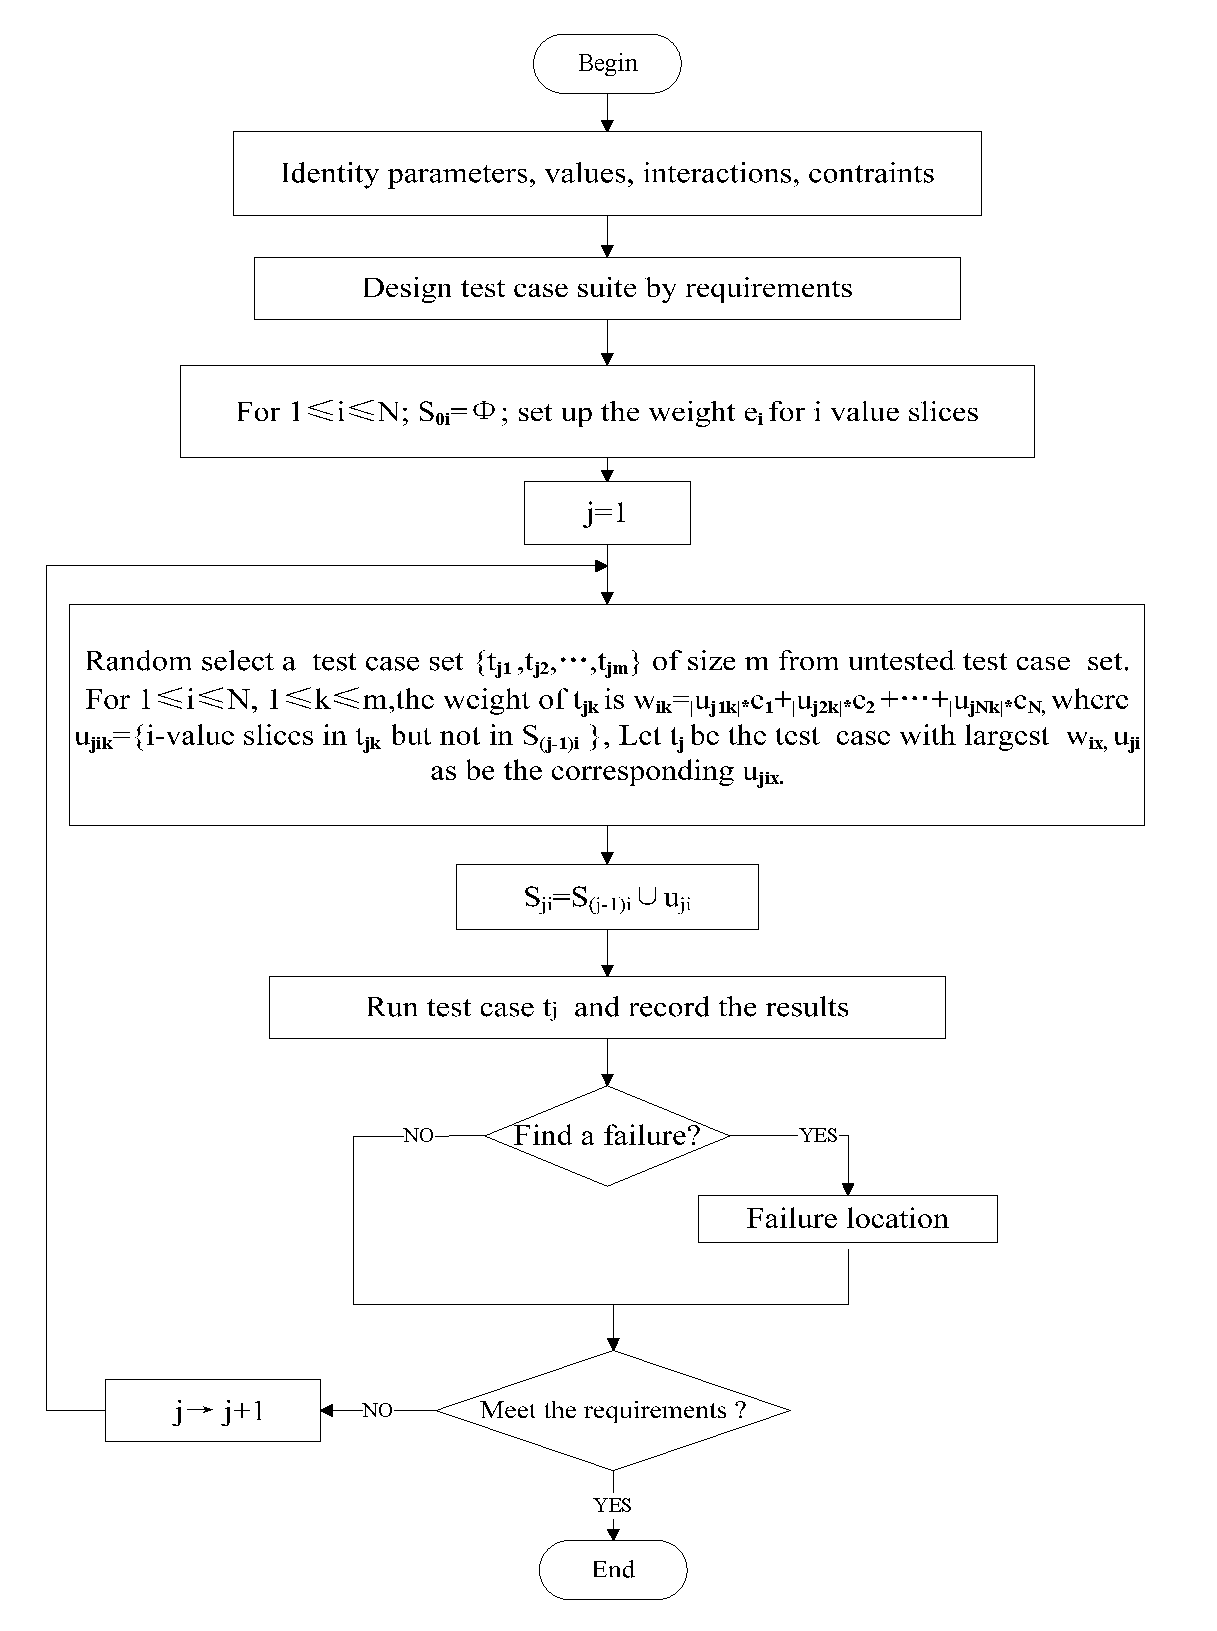
\includegraphics[width=2.5in,height=2.5in]{./CT/CT1.eps}
  \caption{算法一}
  \label{fig:ARCH}
\end{figure}

1 算法简介:

   算法一分别对权值是$weight\_bad$与$weight\_good$进行的两组实验,并将得到的两组实验结果一进行对比。
   
2 算法评价:

   正常情况下,由于$weight\_good$更接近与真实植入的bugs的分布,所以根据$weight\_good$来选择出来的测试用例要优于根据$weight\_bad$选择出来的测试用例,所以在检测出相同的bugs的时候,所用的测试用例越少说明效果越好,我们所期盼的结果是$weight\_good$的实验结果要优于$weight\_bad$的实验结果,并且在每组实验中,m越大实验效果越好。
	\subsubsection{算法二}

算法二流程图\ref{fig:ARCH}
 \begin{figure}[htb]
   \centering
   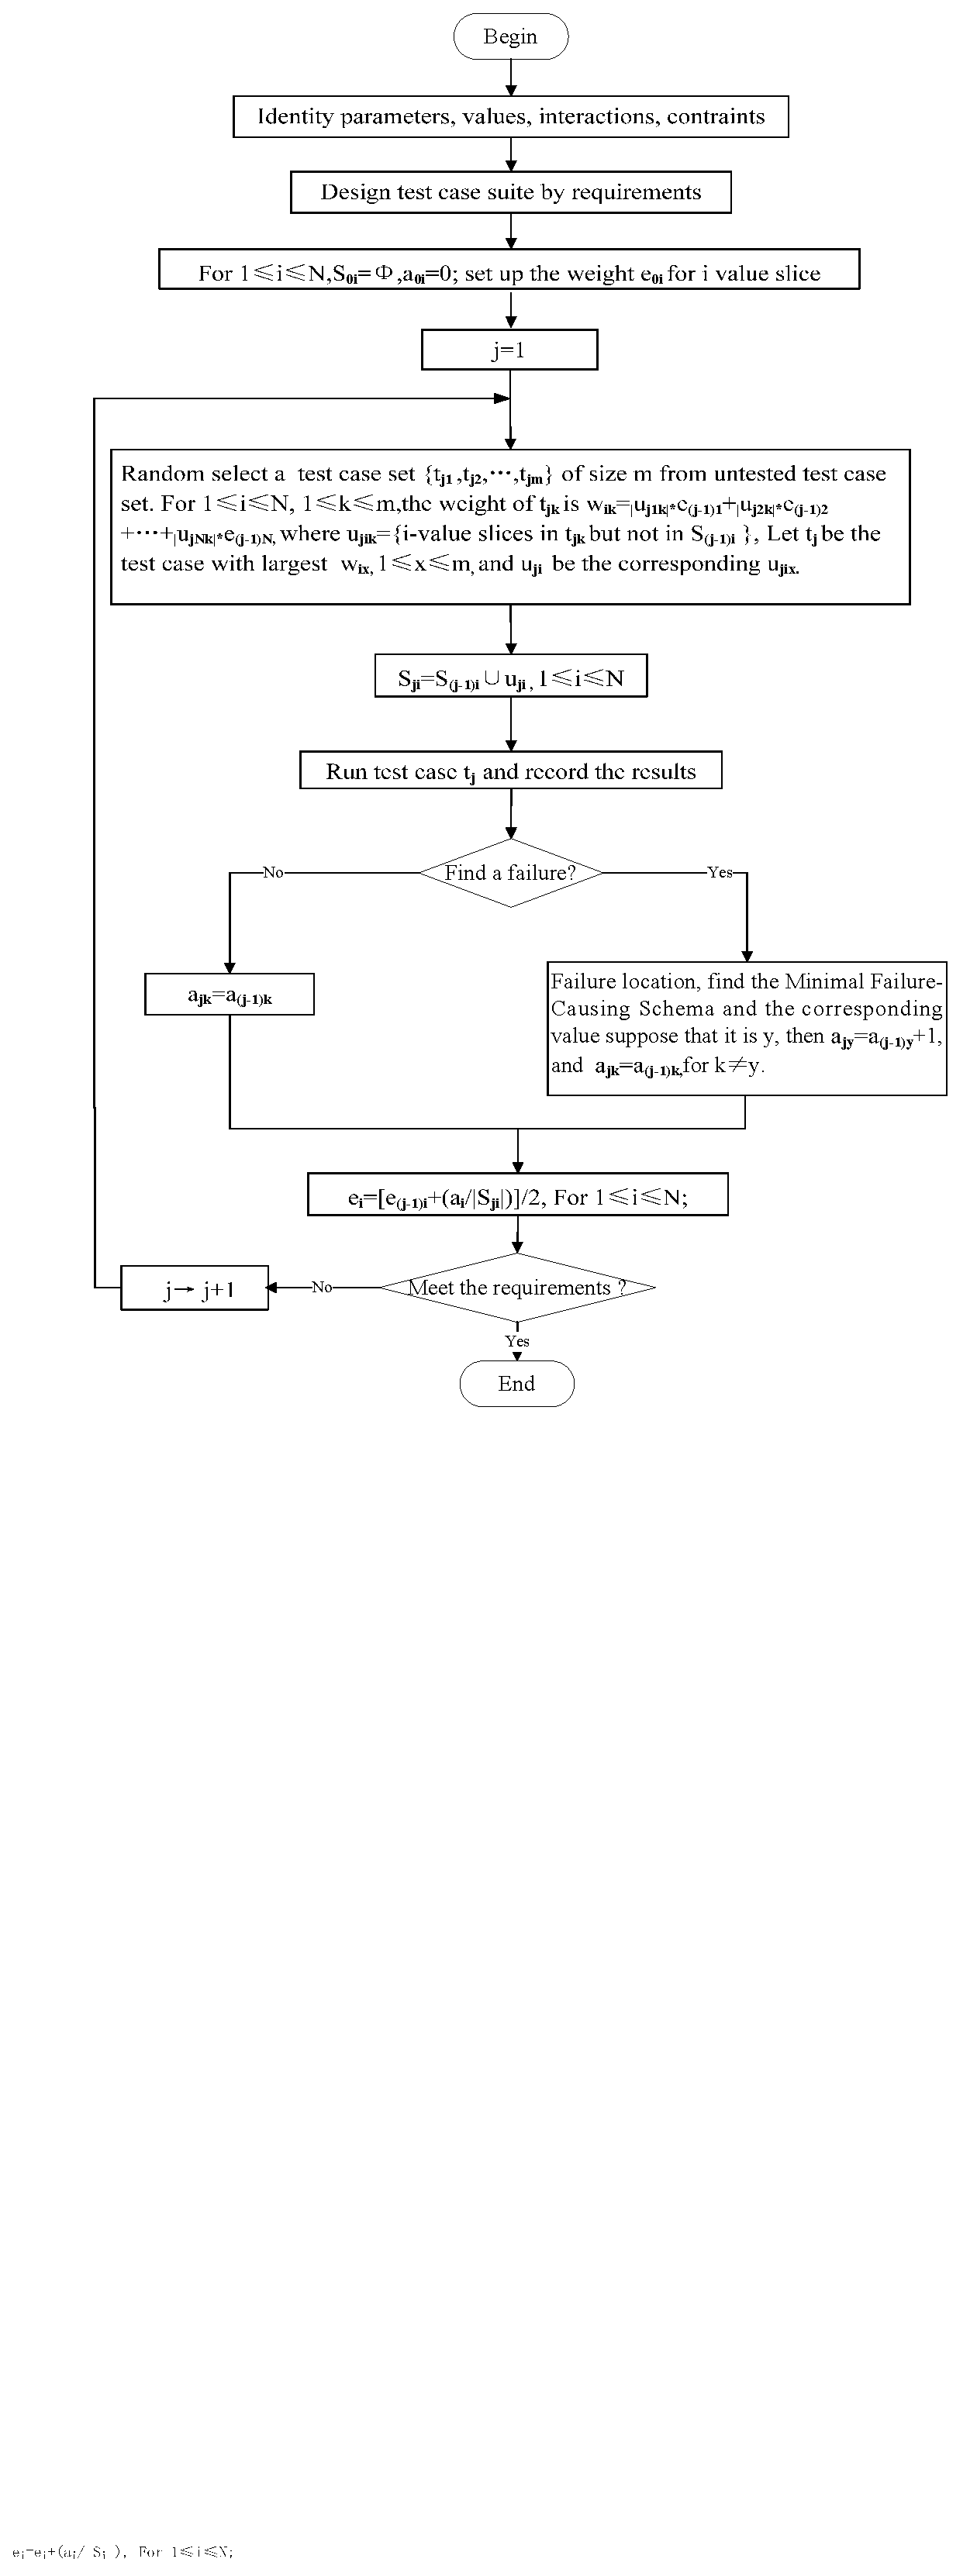
\includegraphics[width=2.5in,height=2.5in]{./CT/CT2.eps}
   \caption{算法二}
   \label{fig:ARCH}
 \end{figure}

1 算法简介:

   算法二是在$weight\_bad$的情况下进行的实验,并对$weight\_bad$进行不端的更新操作,使其越来越接近与真实的权值(最初植入的bugs的分布)
   
2 算法评价:

   首先,在检测出相同bugs的时候用的测试用例越少说明算法越好,而正常情况下m值越大算法的效果越好,再有在权值更新的过程中m值越大权值更新的效果越好即越快速的接近于真实权值。
	\subsubsection{算法三}

算法三流程图\ref{fig:ARCH}
 \begin{figure}[htb]
   \centering
   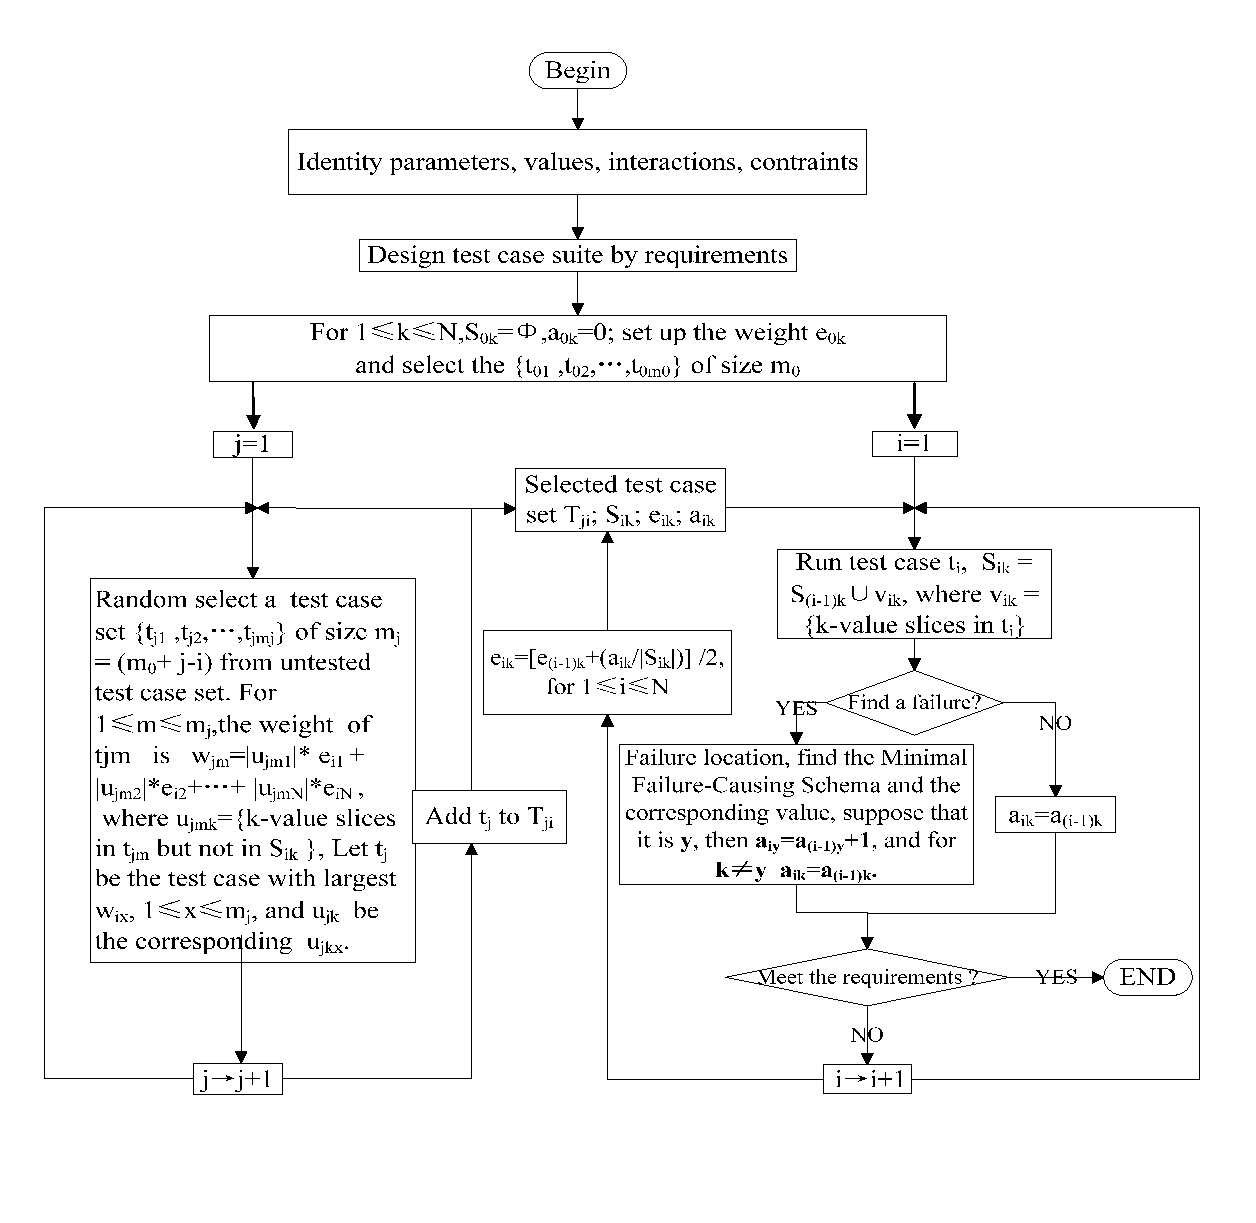
\includegraphics[width=2.5in,height=2.5in]{./CT/CT3.eps}
   \caption{算法三}
   \label{fig:ARCH}
 \end{figure}

1 算法简介:

   并行是指,从m个测试用例中选择一个最好的待测用例与测试这两个过程是并行的。
   
   一,选择最好的测试用例包括两部分:1 通过更新好的权值,计算m个测试用例的检测bugs的效率值,并从中选择一个值为最大的即最好的测试用例作为待测用例。2 将选好的待测用例所新增的$i\_ways$组合数加入程序中定义的相应的$i\_ways$集合中,用于下一次选择待测用例。
   
   二,测试部分,我们模拟真实测试情况,将其赋予一个时间ti。(本次实验ti服从lamda=2的指数分布,即ti的平均值为0.5,方差为0.25)
算法三记录两个时间:1 选择最好的测试用例的时间; 2 测试模块的时间

2 算法评价:

   在检测出相同的bugs的时候,所用的测试用例越好说明算法的效果越好,因为我们是将算法三与算法二进行对比,分别对比两个算法运行的时间和检测bugs的效率。我们所期盼的结果是在检测出相同的bugs的时候算法三用的时间要小于算法二所用的时间,或者是在算法运行相同的时间,检测出来的bugs越多说明算法效率越高,效果越好,这个也是算法三要优于算法二。
\subsection{ 组合覆盖率}
定义,数学公式,性质(组合覆盖率=缺陷的发现率)

$i\_ways$覆盖率的定义:
\begin{equation}
C_i^{(n)}=\frac{m_i(n)}{M_i}
\end{equation}
\\其中$m_i(n)$代表第n个测试用例结束后,已经用到的总的$i\_ways$组合的个数,它是关于n的函数。$M_i$是总的$i\_ways$的组合个数。
\begin{equation}
Coverage_c(n)=C_1^{(n)} \cdot \frac{B_1(n)}{B(n)}+C_2^{(n)} \cdot \frac{B_2(n)}{B(n)}+C_3^{(n)} \cdot \frac{B_4(n)}{B(n)}+C_5^{(n)} \cdot \frac{B_i(n)}{B(n)}...+C_i^{(n)} \cdot \frac{B_i(n)}{B(n)}
\end{equation}
\\其中
\begin{equation}
B(n)= \sum_{i=1}^N B_i(n) 
\end{equation}
\\$B_i(n)$为第n个测试用例结束后,对总的$i\_ways$的缺陷个数的估计值(因为开始时,不知道软件中的缺陷数,所以在测试的过程当中要对总的缺陷数进行估计),$B(n)$为系统当中总的缺陷数(这也是个估计值)。
\\其中$B_i(n)$的计算方式为:$\frac{B_i(n)}{b_i(n)}=\frac{M_i}{m_i(n)}$,由此可得
\begin{equation}
B_i(n)=\frac{M_i}{m_i(n)} \cdot b_i(n)
\end{equation}
\\其中$b_i(n)$是n个测试用例结束后前n个测试用例发现的$i\_ways$总的缺陷数。
\\将公式(1)(4)带入到公式(2)中可以化简得到
\begin{equation}
Coverage_c(n)=\frac{\sum_{i=1}^N b_i(n)}{B(n)}
\end{equation}
\\其中公式(5)的含义是,n个测试用例结束后,组合覆盖率=发现的缺陷的总的个数/估计的总的缺陷数
\\总结:通过以上文档可以看到,首先我们定义了$i\_ways$的覆盖率,然后我们定义了组合覆盖率,根据组合覆盖率的定义我们可以看出,组合覆盖率是通过$i\_ways$的覆盖率乘以其对应的权值,其中$i\_ways$的覆盖率的权值是$i\_ways$检测的缺陷数$B_i(n)$与我们估计的总的缺陷数$B(n)$的比值,这样以来我们就将组合覆盖率与缺陷的发现率联系到了一起,就像我们公式(5)定义的那样。

\begin{itemize}
    \item 1 假设:$i\_ways$缺陷的分布是均匀分布,比较参考Grottke的文章 test affect 2013 PE
    \item 2 remark:组合覆盖率是最合理的覆盖率
\end{itemize}
\subsection{ 算法介绍}
    \subsubsection{ 算法一} 性质(定理),单调性
    \subsubsection*{定理一}
    \begin{thm}
Let $B_i$ represent i\_ways faults, and $M_i$ represent the number of i\_ways combinations.
Let $b_i(n)$ denote the number of faults for i\_ways combination when the $n$ test cases finished testing, 
and  $m_i(n)$ denote the used number of i\_ways combinations when the $n$ test cases finished testing.
The counting process $b_i(n),m_i(n)$ satisfy the following :
$\forall\varepsilon>0$,  
\begin{equation}  
\P(|\frac{b_i(n)}{m_i(n)} - \frac{B_i}{M_i}| \le \varepsilon )
        \geq {1-\frac{1}{m_i(n)\varepsilon}}
\end{equation}
\end{thm}

\begin{proof}
When $n\rightarrow \infty$, it is clear that $ m_i(n)\rightarrow M_i $, and $ b_i(n)\sim \binom{m_i(n)}
{\frac{B_i}{M_i}} $, Chebyshev's inequality gives 

$ 1 \geq P \{\vert \frac{b_i(n)}{m_i(n)} - 
\frac{B_i}{M_i}\vert < \varepsilon \}
\geq 1-\frac{m_i(n)\cdot \frac{B_i}{M_i} \cdot  (1-\frac{B_i}{M_i})}{m_i(n)^2\cdot \varepsilon^2} $
\\Moreover,
$1-\frac{m_i(n)\cdot \frac{B_i}{M_i} \cdot  (1-\frac{B_i}{M_i})}{m_i(n)^2\cdot \varepsilon^2}
\geq 1-\frac{1}{m_i(n) \cdot \varepsilon} $, so that the proof holds. 
\end{proof}

    \subsubsection*{定理2}
设$b_i^{m_1}(n)$ 和$b_i^{m_2}(n)$是算法一最优权值下,参数m分别取值
$m^1,m^2(m^1<m^2)$时,发现的缺陷的总的数目。那么
\begin{equation}  
E(b_i^{m_1}(n)) \leq E(b_i^{m_2}(n))
\end{equation}
\\证明过程:

采用数学归纳法,当n=1时,
可以将从$m^2$个测试用例中选出一个最好的测试用例,检测出来的bugs个数$E(b_i^{m_2}(1))$,看成是先取$m^1$个测试用例,从中选取一个最好的测试用例检测出来的bugs个数$E(b_i^{m_1}(1))$,再取$m^2-m^1$个测试用例,从中选取一个最好的测试用例检测出来的bugs的个数
$E(b_i^{(m_2-m_1)}(1))$,而$E(b_i^{m_2}(1))=E(max\{b_i^{m_1}(1),b_i^{(m_2-m_1)}(1)\})$
所以明显有$E(b_i^{m_1}(1)) < E(b_i^{m_2}(1))$ 。

假设,当$n\leq k$
时有$E(b_i^{m_1}(k)) \leq E(b_i^{m_2}(k))$成立,
那么当$n=k+1$用反正法证明$E(b_i^{m_1}(k+1)) \leq E(b_i^{m_2}(k+1))$

首先假设$E(b_i^{m_1}(k+1)) > E(b_i^{m_2}(k+1))$
设$m=m_1$时,算法2第$k$个测试用力执行后发现的缺陷数是$X_k$, $m=m_2$时算法2第$k$个测试用力执行后发现的缺陷数是$Y_k$, 那么
$b_i^{m_1}(k)=\sum_{n=1}^{k}X_n$, and $b_i^{m_2}(k)=\sum_{n=1}^{k}Y_n$.
我们设$m=m^1$和$m=m^2$时,第k+1次选取出来的最好测试用例检测出来的bugs的个数的期望分别
$E(X(k+1)),E(Y(k+1))$

由于我们假设$E(b_i^{m_1}(k+1)) > E(b_i^{m_2}(k+1))$,
\\即
$E(b_i^{m_1}(k))+E(X(k+1)) > E(b_i^{m_2}(k))+E(Y(k+1))$
第k+1次从$m^1$中选取一个最好的测试用例检测出来的bugs个数的期望为
$E(X(k+1))$ 。我们将$m^1$看成是先取$m^0$ 再取$ m^1-m^0 $ 。
从 $m^0$个测试用例中选取一个最好的测试用例检测出来的bugs个数为
$E(X^{m_0}(k+1))$ 个,
再从 $ m^1-m^0 $ 中选出一个最好的测试用例检测出来的bugs的个数为 
$E(X^{(m_1-m^1_0)}(k+1))$ 个,
其中 $E(X(k+1)) 
=E(max \{X^{m^1_0}(k+1)),X^{(m_1-m^1_0)}(k+1))\} )$。
当$m=m^2$时我们用同样的方法分割选取,
从$m^0$个测试用例中选取最好的测试用例检测出来的bugs的个数的期望为 
$E(Y^{m^2_0}(k+1))$
从$ m^2-m^0 $ 中选出一个最好的测试用例检测出来的bugs的个数的期望为 
$E(Y^{(m_2-m^2_0)}(k+1))$ 个,
其中
$E(Y(k+1))=E(max \{Y^{m^2_0}(k+1),Y^{(m_2-m^2_0)}(k+1))\})$ 
由采样原理可知存在一个$m^0$,使得
$E(b_i^{m_1}(k))+X(k+1) = E(b_i^{m_2}(k))+Y(k+1)$
,那么在K+1次选取的第二阶段$m^1-m^0$,$m^2-m^0$ 。
由于$m^1-m^0<m^2-m^0$
所以有$X^{(m_2-m^2_0)}(k+1)) \leq Y^{(m_2-m^2_0)}(k+1))$ ,
又因为
$E(X(k+1)) 
=E(max \{X^{m^1_0}(k+1)),X^{(m_1-m^1_0)}(k+1))\} )$
\\$E(Y(k+1)) 
=E(max \{Y^{m^1_0}(k+1)),Y^{(m_1-m^1_0)}(k+1))\} )$
\\因为
$E(b_i^{m_1}(k))+X^{m^1_0}(k+1)) = E(b_i^{m_2}(k))+Y^{m^1_0}(k+1))$
\\即
$E(b_i^{m_1}(k)) = E(b_i^{m_2}(k))+ (Y^{m^1_0}(k+1)) - X^{m^1_0}(k+1)))$
\\又因为 
$(Y(k+1)) - X(k+1)))
\geq (Y^{m^1_0}(k+1)) - X^{m^1_0}(k+1)))$
\\所以
$E(b_i^{m_1}(k)) 
\leq  E(b_i^{m_2}(k))+(Y(k+1) - X(k+1))$
\\即
$E(b_i^{m_1}(k))+ X(k+1)) \leq E(b_i^{m_2}(k))+Y(k+1))$
\\即$ E(b_i^{m_1}(k+1)) \leq E(b_i^{m_2}(k+1))$
\\这与假设相矛盾,所以有$\forall n \leq  1 ,E(b_i^{m_1}(k)) \leq E(b_i^{m_2}(k)) $

定理2的物理意义为:算法1在参数m取值$m^1$,$m^2$时($m^1<m^2$),
执行相同的测试用例后,发现的缺陷数目的期望值,m取$m^1$的情况下要小于m取$m^2$,
即m越大,检测缺陷的效果越好。
    \subsubsection{ 算法二}性质(定理),权值收敛,单调性,收敛速度的讨论

The theories of algorithm 1 apply the alogorithm 2 and 3. 
The updating weight 1:
\begin{thm}
\begin{equation} 
\rho _i(k+1)= \frac{\rho_i(k)+\frac {b_i(k+1)}{m_i(k+1)}}{2} \rightarrow  \frac{B_i}{M_i}
\end{equation}
\end{thm}

\begin{proof}
$\rho_i(1)= \frac{\rho_i(0)+\frac {b_i(1)}{m_i(1)}}{2}
=\frac{1}{2}\rho_i(0)+\frac{1}{2}\frac{b_i(1)}{m_i(1)}$
\\$\rho_i(2)= \frac{\rho_i(1)+\frac {b_i(2)}{m_i(2)}}{2}
=\frac{1}{2^2}\rho_i(0)+\frac{1}{2^2}\frac{b_i(1)}{m_i(1)}
+\frac{1}{2}\frac{b_i(2)}{m_i(2)}$.
And also, we obtain  $\rho_i(n)= \frac{\rho_i(n-1)+\frac {b_i(n)}{m_i(n)}}{2}
=\frac{1}{2^n}\rho_i(0)+\frac{1}{2^n}\frac{b_i(1)}{m_i(1)}
+\frac{1}{2^{n-1}}\frac{b_i(2)}{m_i(2)}+……+\frac{1}{2}\frac{b_i(n)}{m_i(n)}$.
From the following lemma we conclude $\rho_i(n)\rightarrow\frac{B_i}{M_i}$
\end{proof}

\begin{lemma}
For sequences $P_1,P_2.....P_n$
satisfying $ \lim \frac{P_n}{P_1+P_2+......+P_n} \rightarrow 0 $.
If $\lim a_n \rightarrow a$,
then $\lim \frac{a_n \cdot P_1+a_{n-1} \cdot P_2+...+a_1\cdot P_n}{P_1+P_2+......+P_n}=a$
\end{lemma}

\begin{proof}
Because $\lim a_n \rightarrow a$
so that $\forall \varepsilon,\exists N_1$,
for all $n>N_1$, there exsits an equation 
$|a_n-a|<\frac{\varepsilon}{3}$,
and also $\{a_n\}$ is bounded, there $\exists M>0$, which makes $|a_n|<M$.
For a sequence $\{P_1,P_2.....P_n\}$,
satisfying $\lim \frac{P_n}{P_1+P_2+......+P_n} \rightarrow 0$.
For all the above $\varepsilon$,there exists $N_2$,which make when $n>N_2$,
$|\frac{P_n}{P_1+P_2+......+P_n}-0| \leq \frac{\varepsilon}{3MN_1}$,
pick up $N_3>max\{N_1,N_2\}$,
and make three segments for $n$, so that we have 
\begin{eqnarray*}
| \frac{a_n P_1+a_{n-1} P_2+...+a_1 P_n}{P_1+P_2+......+P_n}-a| \\
=( \frac{|a_1-a| P_n+|a_2-a| P_{n-2}+...+|a_n-a| P_1}{P_1+P_2+......+P_n})\\
\leq ( \frac{|a_1-a| P_n+|a_2-a| P_{n-2}+...+|a_{N_1}-a| P_{n-N_1+1}}{P_1+P_2+......+P_n})\\
+ ( \frac{|a_{N_1+1}-a| P_{n-N_1}+...+|a_{n-N_3}-a|  P_{N_3+1}}{P_1+P_2+......+P_n})\\
+ ( \frac{|a_{n-N_3+1}-a|  P_{N_3}+...+|a_{n}-a| P_1}{P_1+P_2+......+P_n})       
\end{eqnarray*}
\\Since ${a_n}$ is bounded,$\forall n,\exists M>0$
makes $|a_n-a|<M$
\begin{eqnarray*}
( \frac{|a_1-a| P_n+|a_2-a| P_{n-2}+...+|a_{N_1}-a| P_{n-N_1+1}}{P_1+P_2+......+P_n})\\
\leq M.\frac{P_n+...+P_{n-N_1+1}}{P_1+P_2+...+P_n} \leq N_1 \cdot M \cdot \frac{\varepsilon}{3MN_1}
=\frac{\varepsilon}{3}
\end{eqnarray*}
\begin{eqnarray*}
( \frac{|a_{N_1+1}-a| P_{n-N_1}+...+|a_{n-N_3}-a|  P_{N_3+1}}{P_1+P_2+......+P_n})\\
    \leq(\frac{P_{n-N_1}+...+P_{N_3+1}}{P_1+P_2+...+P_n}
\cdot \frac{\varepsilon}{3})
    \leq \frac{\varepsilon}{3}
\end{eqnarray*}
\begin{eqnarray*}
( \frac{|a_{n-N_3+1}-a|  P_{N_3}+...+|a_{n}-a| P_1}{P_1+P_2+......+P_n}) \leq \\
(\frac{P_{N_3}+...+P_1}{P_1+P_2+...+P_n} \cdot \frac{\varepsilon}{3}) \leq \frac{\varepsilon}{3}
\end{eqnarray*}
\begin{equation}  
 \forall n>N_3, | \frac{a_n P_1+a_{n-1} P_2+...+a_1 P_n}{P_1+P_2+......+P_n}-a|\leq \varepsilon 
\end{equation}
\\We conclude this lemma. 
\end{proof}

\subsubsection*{定理6}
权值调整方法2:
\begin{equation}  
 \begin{aligned}
 & \rho_i(k+1)=\frac{1\cdot\rho_i(0)+...+k\cdot\rho_i(k-1)}
   {\frac{(k+2)(k+3)}{2}}+\\
 & \frac{(k+1)\cdot\rho_i(k)+ (k+2)\cdot\frac{b_i(k+1)}{m_i(k+1)}}
   {\frac{(k+2)(k+3)}{2}}\\
&\rho_i(k+1)\rightarrow \frac{B_i}{M_i}
 \end{aligned}
\end{equation}
\\证明过程:
\\$\rho_i(1)=\frac{\rho_i(0)+2\frac{b_i(1)}{m_i(1)}}{\frac{2.3}{2}}=\frac{1}{3}\rho_i(0)+\frac{2}{3}\frac{b_i(1)}{m_i(1)}=a_i^1(0)\rho_i(0)+a_i^1\frac{b_i(1)}{m_i(1)}$
\\$\rho_i(2)=\frac{\rho_i(0)+2\rho_i(1)+3\frac{b_i(1)}{m_i(1)}}{\frac{3.4}{2}}=a_i^2(0)\rho_i(0)+a_i^2\frac{b_i(1)}{m_i(1)}+a_i^2(2)\frac{b_i(2)}{m_i(2)}$
\\设$\rho_i(n)=a_i^n(0)\rho_i(0)+a_i^n(1)\frac{b_i(1)}{m_i(1)}+a_i^n(2)\frac{b_i(2)}{m_i(2)}+...+a_i^n(n)\frac{b_i(n)}{m_i(n)}$
\\其中参数经过数学计算处理得到:
$ \begin{displaymath}
   a_i^n(k) = \left\{
     \begin{array}{lr}
       \frac{2}{k+2}  & n = k\\
       \frac{4(k+1)}{(k+2)^2(k+3)} & n=k+1 \\
       \frac{n+3}{n+1}\frac{4(k+1)}{(k+4)(k+3)(k+2)} & n>k+1
     \end{array}
   \right.
\end{displaymath}$
\\令$P_k=a_i^n(n-k)$
\\则$\rho_i(n)=P_n\rho_i(0)+P_{n-1}\frac{b_i(1)}{m_i(1)}+P_{n-2}\frac{b_i(2)}{m_i(2)}+...+P_0\frac{b_i(n)}{m_i(n)}$
\\其中系数$P_1,P_2...P_n$满足$\lim \frac{P_n}{P_1+P_2+......+P_n} \rightarrow 0$,即$\rho_i(n)$满足引理四,所以有$\rho_i(n)\rightarrow \frac{B_i}{M_i}$

\subsubsection*{定理六具体证明过程}
\begin{equation}  
\rho_i(k+1)=\frac{1\cdot\rho_i(0)+...+k\cdot\rho_i(k-1)+(k+1)\cdot\rho_i(k)+(k+2)\cdot\frac{b_i(k+1)}{m_i(k+1)}}{\frac{(k+2)(k+3)}{2}}
\end{equation}
\\证明过程:
\\$\rho_i(1)=\frac{\rho_i(0)+2\frac{b_i(1)}{m_i(1)}}{\frac{2.3}{2}}=\frac{1}{3}\rho_i(0)+\frac{2}{3}\frac{b_i(1)}{m_i(1)}=a_i^1(0)\rho_i(0)+a_i^1\frac{b_i(1)}{m_i(1)}$
\\$\rho_i(2)=\frac{\rho_i(0)+2\rho_i(1)+3\frac{b_i(1)}{m_i(1)}}{\frac{3.4}{2}}=a_i^2(0)\rho_i(0)+a_i^2\frac{b_i(1)}{m_i(1)}+a_i^2(2)\frac{b_i(2)}{m_i(2)}$
\begin{equation}
\rho_i(n)=a_i^n(0)\rho_i(0)+a_i^n(1)\frac{b_i(1)}{m_i(1)}+a_i^n(2)\frac{b_i(2)}{m_i(2)}+...+a_i^n(n)\frac{b_i(n)}{m_i(n)}
\end{equation}
\\将(7)公式中的n分别取值0,1,2,3.......k,分别得到
$\rho_i(0),\rho_i(1),\rho_i(2),\rho_i(3).....\rho_i(k+1)$,
然后带入到公式(6)中,并得到等号两边对应系数相等,
$\rho_i(0)$的系数对应相等将会得到
$a_i^n(0)=\frac{1+2a_i^1(0)+3a_i^2(0)+...+na_i^{n-1}(0)}{\frac{(n+1)(n+2)}{2}}$
\\${\frac{(n+1)(n+2)}{2}}a_i^n(0)={1+2a_i^1(0)+3a_i^2(0)+...+na_i^{n-1}(0)}$
\\将上式的n取n+1将会得到
\\${\frac{(n+2)(n+3)}{2}}a_i^{n+1}(0)={1+2a_i^1(0)+3a_i^2(0)+...+na_i^{n-1}(0)+(n+1)a_i^n(0)}$ 
\\将上边两式做减法将会得到
\\${\frac{(n+2)(n+3)}{2}}a_i^{n+1}(0)-{\frac{(n+1)(n+2)}{2}}a_i^n(0)=(n+1)a_i^n(0)$
\\整理得到$a_i^{n+1}(0)=\frac{(n+1)(n+4)}{(n+2)(n+3)}a_i^n(0)$
\\$a_i^1(0)=\frac{1}{3},a_i^2(0)=\frac{2 \cdot 5}{3 \cdot 4} \cdot \frac{1}{3}$
\\$a_i^3(0)=\frac{3 \cdot 6}{4 \cdot 5 } \cdot \frac{2 \cdot 5}{3 \cdot 4} \cdot \frac{1}{3}
=\frac{6}{4} \cdot \frac{2}{4} \cdot \frac{1}{3}$
\\$a_i^4(0)=\frac{4 \cdot 7}{5 \cdot 6 } \cdot \frac{6 \cdot 2}{4 \cdot 4} \cdot \frac{1}{3}
=\frac{7}{5} \cdot \frac{2}{4} \cdot \frac{1}{3}$
\\同理得
\\$a_i^n(0)=\frac{(n+3)}{(n+1)} \cdot \frac{2}{4} \cdot a_i^1(0)$
\\同上,再处理$a_i^n(1)$

$\frac{b_i(1)}{m_i(1)}$的系数对应相等将会得到
\\$a_i^n(1)=\frac{2a_i^1(1)+3a_i^2(1)+...+na_i^{n-1}(1)}{\frac{(n+1)(n+2)}{2}}$
\\${\frac{(n+1)(n+2)}{2}}a_i^n(1)={2a_i^1(1)+3a_i^2(1)+...+na_i^{n-1}(1)}$
\\同样将上式n取n+1得到
\\$\frac{(n+2)(n+3)}{2}a_i^{n+1}(1)=2a_i^1(1)+3a_i^2(1)+...+na_i^{n-1}(1)+(n+1)a_i^{n}(1)$
\\两式相减得到$a_i^{n+1}(1)=\frac{(n+1)(n+4)}{(n+2)(n+3)}a_i^n(1)$
\\$a_i^1(1)=\frac{2}{3},a_i^2(1)=\frac{2a_i^1(1)}{\frac{3 \cdot 4}{2}}=\frac{2}{9}$
\\$a_i^3(1)=\frac{3 \cdot 6}{4 \cdot 5 }  \cdot \frac{2}{9}
=\frac{1}{5}$
\\$a_i^4(1)=\frac{4 \cdot 7}{5 \cdot 6 } \cdot \frac{1}{5}$
\\同理得到:
\\$a_i^n(1)=\frac{3}{5} \cdot \frac{(n+3)}{(n+1)} \cdot \frac{2}{9} \cdot a_i^2(1)
=\frac{2}{15} \cdot \frac{(n+3)}{(n+1)} \cdot a_i^2(1)$
\\再用同样的方式处理$a_i^n(2)$,最后得到
\\$a_i^n(1)=\frac{(n+3)}{(n+1)} \cdot \frac{4}{6} \cdot a_i^3(2)$
\\递归得出
\\$a_i^n(k)=\frac{(n+3)}{(n+1)} \cdot \frac{(k+2)}{k+4} \cdot a_i^{k+1}(k)$

即
$ \begin{displaymath}
   a_i^n(k) = \left\{
     \begin{array}{lr}
       \frac{2}{k+2}  & n = k\\
       \frac{4(k+1)}{(k+2)^2(k+3)} & n=k+1 \\
       \frac{n+3}{n+1}\frac{4(k+1)}{(k+4)(k+3)(k+2)} & n>k+1
     \end{array}
   \right.
\end{displaymath}$

令$P(k)=a_i^n(n-k)$
\begin{equation}
\rho_i(n)=P(n)\rho_i(0)+P(n-1)\frac{b_i(1)}{m_i(1)}+P(n-2)\frac{b_i(2)}{m_i(2)}+...+P(0)\frac{b_i(n)}{m_i(n)}
\end{equation}
\\其中
\\$\frac{P(n)}{P(0)+P(1)+P(2)+....P(n)}
\\=\frac{\frac{n+3}{n+2}\cdot \frac{4(k+1)}{(k+4)(k+3)(k+2)}}{\frac{2}{k+2}+\frac{4(k+1)}{(k+2)^2(k+3)}+\frac{k+5}{k+4}\cdot \frac{4(k+1)}{(k+4)(k+3)(k+2)}+....+\frac{n+3}{n+2}\cdot\frac{4(k+1)}{(k+4)(k+3)(k+2)}}
\\=\frac{\frac{n+3}{n+2}\cdot \frac{4(k+1)}{(k+4)(k+3)(k+2)}}{\frac{2}{k+2}+\frac{4(k+1)}{(k+2)^2(k+3)}+\frac{4(k+1)}{(k+4)(k+3)(k+2)}\cdot(\frac{k+5}{k+4}+\frac{k+6}{k+5})+\frac{k+7}{k+6}+....+\frac{n+3}{n+2}}\rightarrow 0$
\\由引理四可知定理6收敛

\subsubsection*{错误权值更新方式}
\begin{equation}
\rho_i(k+1)=\frac{\rho_i(0)+\rho_i(1)+\rho_i(2)+\rho_i(3)+....\rho_i(k)+\frac{b_i(k+1)}{m_i(k+1)}}{(k+2)}
\end{equation}
$\\ \rho_i(1)=\frac{\rho_i(0)+\frac{b_i(1)}{m_i(1)}}{2}
=\frac{1}{2} \cdot \rho_i(0)+\frac{1}{2} \cdot \frac{b_i(1)}{m_i(1)}
=a_i^1(0)\rho_i(0)+a_i^1(1) \frac {b_i(1)}{m_i(1)}
\\ \rho_i(2)=\frac{\rho_i(0)+\rho_i(1)+\frac{b_i(2)}{m_i(2)}}{3}
=a_i^2(0)\rho_i(0)+a_i^2(1) \frac {b_i(1)}{m_i(1)}+a_i^2(2)\frac{b_i(2)}{m_i(2)}
\\ \rho_i(3)=\frac{\rho_i(0)+\rho_i(1)+\rho_i(2)\frac{b_i(3)}{m_i(3)}}{4}
=a_i^3(0)\rho_i(0)+a_i^3(1) \frac {b_i(1)}{m_i(1)}+a_i^3(2)\frac{b_i(2)}{m_i(2)}+a_i^3(3)\frac{b_i(3)}{m_i(3)}$
\\由上可得:
\begin{equation}
\rho_i(n)=\frac{\rho_i(0)+\rho_i(1)+...+\rho_i(2)\frac{b_i(n)}{m_i(n)}}{(n+1)}
=a_i^n(0)\rho_i(0)+a_i^n(1) \frac {b_i(1)}{m_i(1)}+a_i^n(2)\frac{b_i(2)}{m_i(2)}+a_i^n(3)\frac{b_i(3)}{m_i(3)}+....+a_i^n(n)\frac{b_i(n)}{m_i(n)}
\end{equation}
\\将上述公式中n分别取0,1,2....k+1,带入到公式(8)中,将会得到等式两边对应的
$\\ \frac{b_i(1)}{m_i(1)},\frac{b_i(2)}{m_i(2)},\frac{b_i(3)}{m_i(3)}....\frac{b_i(1)}{m_i(k+1)}$
系数分别相等\\首先处理
$a_i^n(0),a_i^0(0)=\frac{1}{2},a_i^1(0)=\frac{1}{2}
\\a_i^n(0)=\frac{a_i^0(0)+a_i^1(0)+a_i^2(0)+...+a_i^{n-1}(0)}{(n+1)}
\\{(n+1)}a_i^n(0)={a_i^0(0)+a_i^1(0)+a_i^2(0)+...+a_i^{n-1}(0)}
\\{(n+2)}a_i^{n+1}(0)={a_i^0(0)+a_i^1(0)+a_i^2(0)+...+a_i^n(0)}$
\\上边两式相减得到
$a_i^{n+1}(0)=a_i^n(0)=\frac{1}{2}$
\\再处理
$a_i^n(1)$
$a_i^n(1)=\frac{a_i^1(1)+a_i^2(1)+...+a_i^{n-1}(1)}{(n+1)}$
\\${(n+1)}a_i^n(1)=a_i^1(1)+a_i^2(1)+...+a_i^{n-1}(1)$
\\${(n+2)}a_i^{n+1}(1)=a_i^1(1)+a_i^2(1)+...+a_i^{n}(1)$
\\上边两式相减,得到
$a_i^{n+1}(1)=a_i^n(1)=\frac{1}{6}$
\\用同样的方法我们可以求得
$a_i^{n+1}(n-1)=\frac{a_i^n(n-1)}{n+1}=\frac{1}{(n+1) \cdot n}
\\a_i^n(n)=\frac{1}{n+1}$
\\所以有公式(9)其中
$\\a_i^n(0)=\frac{1}{1 \cdot 2},a_i^n(1)=
\frac{1}{2 \cdot 3},a_i^n(2)=\frac{1}{3 \cdot 4}....a_i^n(n-1)
=\frac{1}{n \cdot (n+1)},a_i^n(n)=\frac{1}{n+1}
\\p(k)=a_i^n(n-k)
\frac{b_i(n)}{m_i(n)} \rightarrow \frac{B_i}{M_i}
\frac{P(n)}{P(1)+P(2)+...+P(n)}=
\frac{\frac{1}{2}}{\frac{1}{1 \cdot 2}+\frac{1}{2 \cdot 3}+\frac{1}{3 \cdot 4}+...
+\frac{1}{n \cdot n+1}+\frac{1}{1 \cdot n}} \rightarrow \frac{1}{2}$
\\所以这种权值更新的方法并不能符合引理四的初始条件,所以这种更新权值的方式是错误的
    \subsubsection{ 算法三}性质(定理),权值收敛,单调性,m值的意义,m大小的讨论
\subsection{实验}LiuChao 2006 TSE
	\subsubsection{实验一}
1 算法简介:

	算法一分别对权值是$weight\_bad$与$weight\_good$进行的两组实验,并将得到的两组实验结果一进行对比。
\\2 算法评价:

	正常情况下,由于$weight\_good$更接近与真实植入的bugs的分布,所以根据$weight\_good$来选择出来的测试用例要优于根据$weight\_bad$选择出来的测试用例,所以在检测出相同的bugs的时候,所用的测试用例越少说明效果越好,我们所期盼的结果是$weight\_good$的实验结果要优于$weight\_bad$的实验结果,并且在每组实验中,m越大实验效果越好。
\\3 覆盖率:

	覆盖率是个关于n的函数,其中n是所用到测试用例的个数

	在测试第n个测试用例后,$i\_ways$覆盖率=(已用到的$i\_ways$组合数)/(总的$i\_ways$组合数)

	在测试第n个测试用例后,经过化简得到,组合覆盖率=(以测试出来的bugs的数量)/(估计的bugs的总数量),他们都是关于n的函数。
\\4 评价标准:第一种带权值,第二种不带权值

4.1 评价标准1:

	1*C1+2*C2+3*C3+........+20000*C20000,其中1,2,3,,,,20000代表横坐标,C1,C2,C3,,,,,C20000代表横坐标对应的纵坐标
\\4.2评价标准2:

	C1+C2+C3+......+C20000,其中C1,C2,C3,,,,,C20000代表横坐标对应的纵坐标
\\5 实验部分

5.1 数据准备:

	$bugs\_size$ = [8, 65,78, 68, 35, 1, 0, 0, 0, 0, 0, 0, 0]   

	$bugs\_size$:软件最初植入的Bugs的个数,1-ways错误8个,2-ways错误65个.....一共255个Bugs

	$weight\_good$ = [9, 67, 76, 66, 37, 1] 

	$weight\_bad$ = [10, 170,70,8, 0, 0]

	weight权值是我们凭借经验对未知软件中错误个数的猜测值,$weight\_good$是接近于软件实际含有错误的个数,$weight\_bad$是偏离真实情况的一种估计
\\5.2 实验数据:   
 
	$modules\_size$ = [4, 2, 6, 7, 3, 6, 2, 3, 10, 4, 5, 5, 3] 

	$test\_cases$:共 108864000

	其中,$modules\_size$表示:该测试集有13个参数,第一个参数有4种取值,第二个参数有2中取值,第三个参数有6种取值,第四个参数有7种取值.....该测试用例集一共可以组成108864000个测试用例。
\\5.3 试验结果:

%Good Distribution\ref{fig:ARCH}
 \begin{figure}[htb]
   \centering
   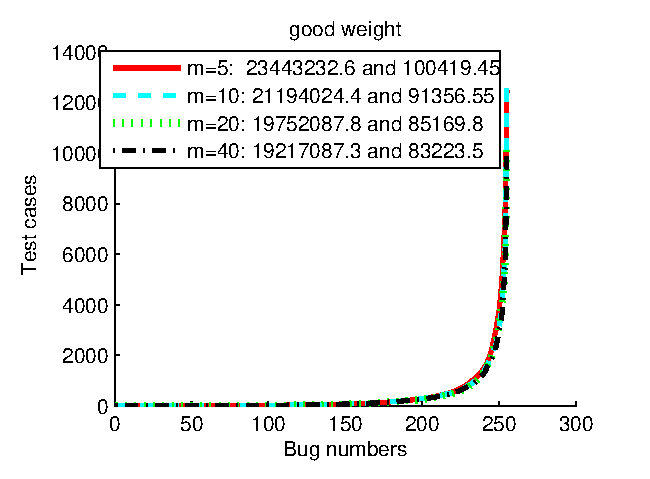
\includegraphics[width=2.5in,height=2.5in]{./a1_picture/good.eps}
   \caption{Good Distribution}
   \label{fig:ARCH}
 \end{figure}
%Bad Distribution\ref{fig:ARCH}
 \begin{figure}[htb]
   \centering
   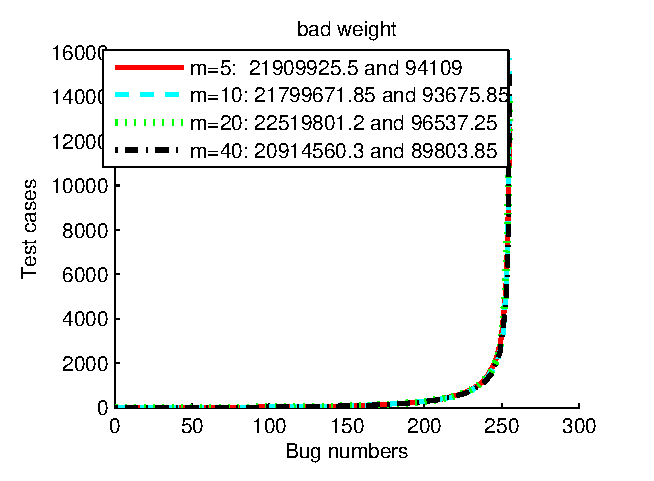
\includegraphics[width=2.5in,height=2.5in]{./a1_picture/bad.eps}
   \caption{Bad Distribution}
   \label{fig:ARCH}
 \end{figure}
%Good and Bad\ref{fig:ARCH}
 \begin{figure}[htb]
   \centering
   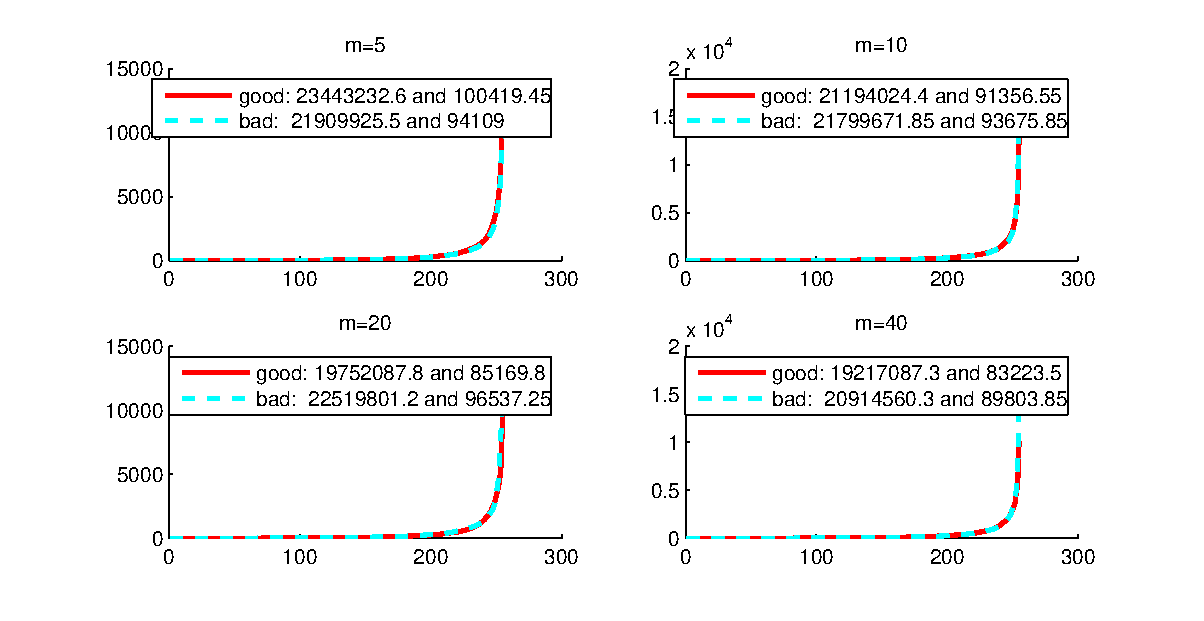
\includegraphics[width=2.5in,height=2.5in]{./a1_picture/good_and_bad.eps}
   \caption{Good and Bad}
   \label{fig:ARCH}
 \end{figure}

5.4.1实验总结:

1 在$weight\_good$ 的情况下,试验结果与我们预先期盼的一样

2 在$weight\_bad$ 的情况下,m=20的时候最不好,其他的m值所对应的结果与我们期盼的也一致

3 在$weight\_good$和$weigh\_bad$对比的实验中,只有m=5的时候不是我们所期盼的结果$weight\_bad$优于$weight\_good$。

%Combination coverage good\ref{fig:ARCH}
 \begin{figure}[htb]
   \centering
   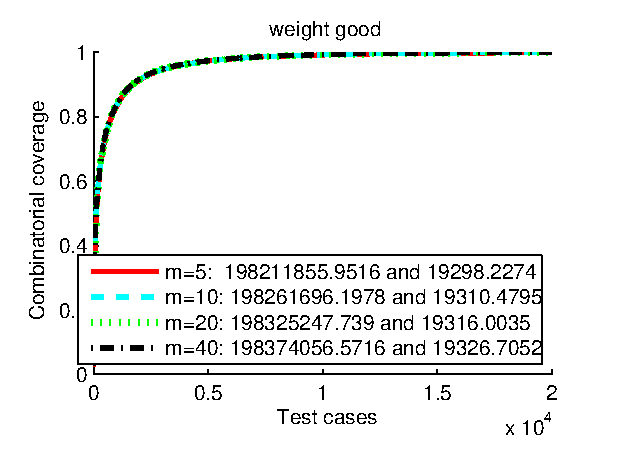
\includegraphics[width=2.5in,height=2.5in]{./a1_picture/combination_coverage_good.eps}
   \caption{Combination coverage good}
   \label{fig:ARCH}
 \end{figure}
%Combination coverage bad\ref{fig:ARCH}
 \begin{figure}[htb]
   \centering
   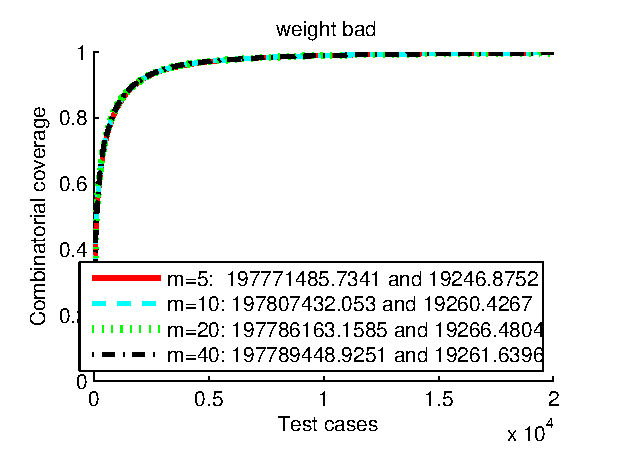
\includegraphics[width=2.5in,height=2.5in]{./a1_picture/combination_coverage_bad.eps}
   \caption{Combination coverage bad}
   \label{fig:ARCH}
 \end{figure}
%i ways combinatio coverage good\ref{fig:ARCH}
 \begin{figure}[htb]
   \centering
   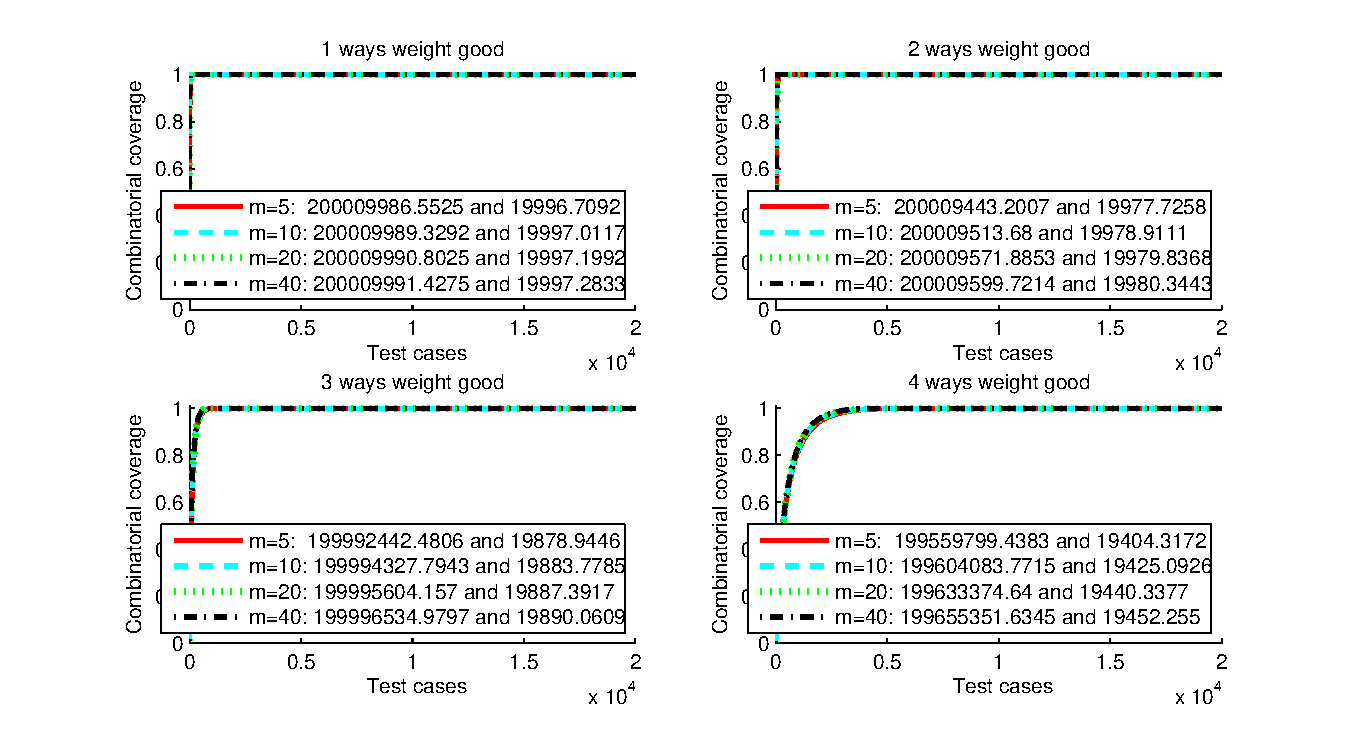
\includegraphics[width=2.5in,height=2.5in]{./a1_picture/i_ways_combinatio_coverage_good.eps}
   \caption{i ways combinatio coverage good}
   \label{fig:ARCH}
 \end{figure}
%i ways combinatio coverage bad\ref{fig:ARCH}
 \begin{figure}[htb]
   \centering
   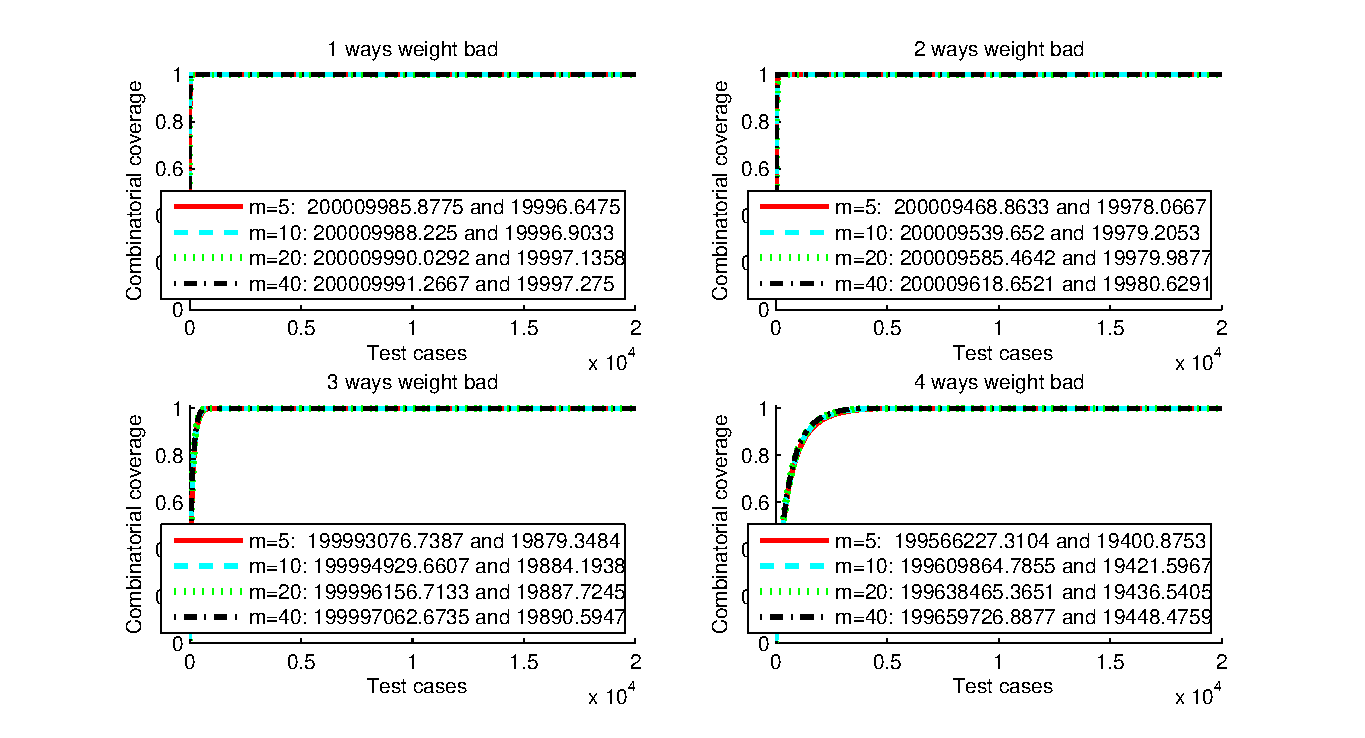
\includegraphics[width=2.5in,height=2.5in]{./a1_picture/i_ways_combinatio_coverage_bad.eps}
   \caption{i ways combinatio coverage bad}
   \label{fig:ARCH}
 \end{figure}
%combination coverage good and bad\ref{fig:ARCH}
 \begin{figure}[htb]
   \centering
   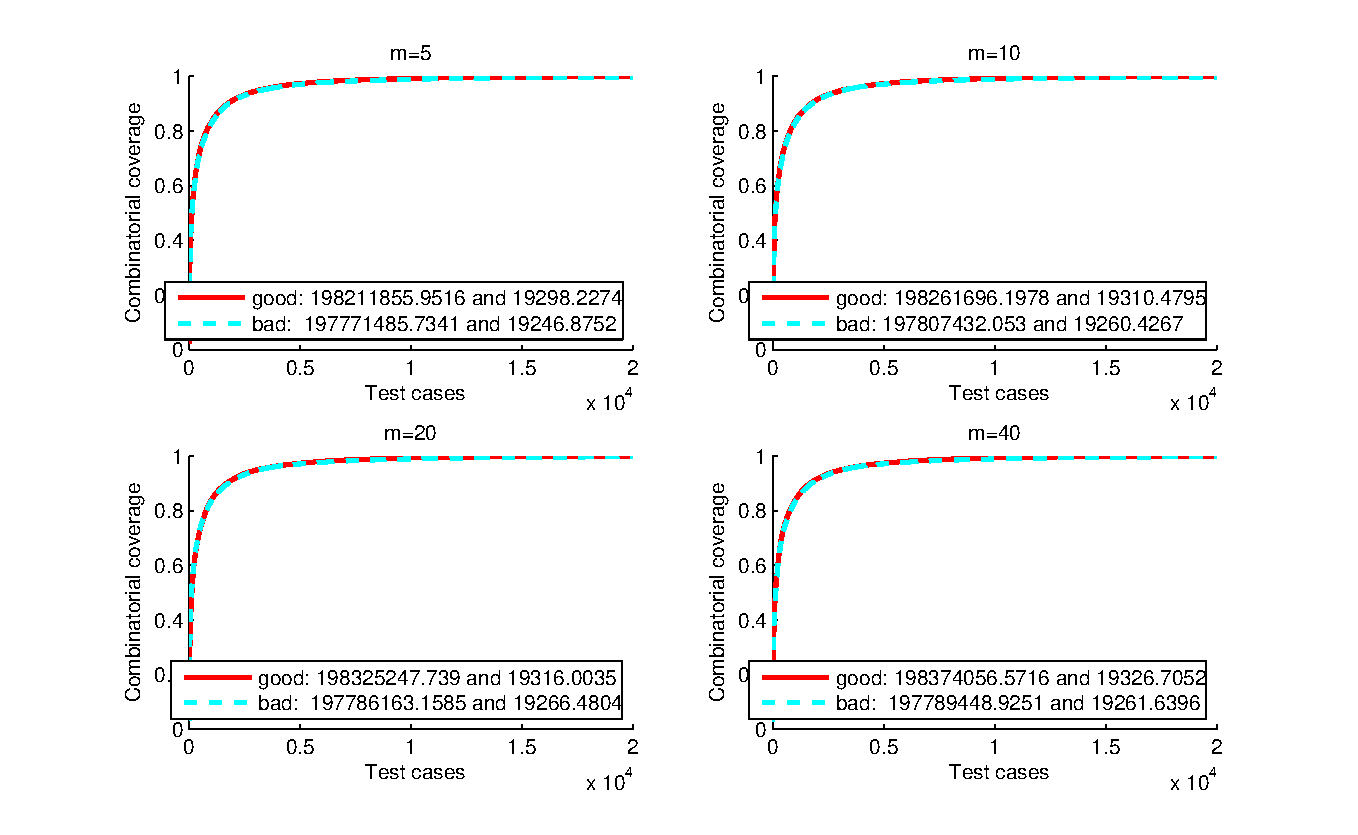
\includegraphics[width=2.5in,height=2.5in]{./a1_picture/combination_coverage_good_and_bad.eps}
   \caption{combination coverage good and bad}
   \label{fig:ARCH}
 \end{figure}

5.4.2实验总结:

1 这次试验图像的横坐标为testcases 纵坐标为coverage ,测试20000个测试用例作为实验结束条件。

2 在计算评价标准的时候,计算的是图像与X轴围成的面积,并且是先求出20组数据的平均值根据平均值绘制出来的图像计算的评价标准(以往的实验也是这么计算的),而不是计算每一组数据的的评价标准然后再取20组的评价标准的平均值,也不是计算与Y轴围成的面积(与Y轴围成的面积计算不了)。

3 根据评价标准来看,$weight\_good$的时候符合老师的要求,m越大,评价标准值越大,即组合覆盖率越好,在$weight\_bad$的时候,两种评价标准却显出了不同的结果,并且差异很大

4 在对比$weight\_good$与$weight\_bad$的情况,m固定,对比$i\_ways$覆盖率等情况都是我们所期盼的。

	\subsubsection{实验二}
1 算法简介: 

	算法二是在$weight\_bad$的情况下进行的实验,并对$weight\_bad$进行不端的更新操作,使其越来越接近与真实的权值(最初植入的bugs的分布)。
\\2 算法评价: 

	首先,在检测出相同bugs的时候用的测试用例越少说明算法越好,而正常情况下m值越大算法的效果越好,再有在权值更新的过程中m值越大权值更新的效果越好即越快速的接近于真实权值。
\\3 覆盖率:

	覆盖率是个关于n的函数,其中n是所用到测试用例的个数

	在测试第n个测试用例后,$i\_ways$覆盖率=(已用到的$i\_ways$组合数)/(总的$i\_ways$组合数)

	在测试第n个测试用例后,经过化简得到,组合覆盖率=(以测试出来的bugs的数量)/(估计的bugs的总数量),他们都是关于n的函数。
\\4 评价标准:第一种带权值,第二种不带权值
\\4.1 评价标准1:

	1*C1+2*C2+3*C3+........+20000*C20000,其中1,2,3,,,,20000代表横坐标,C1,C2,C3,,,,,C20000代表横坐标对应的纵坐标
\\4.2评价标准2:

	C1+C2+C3+......+C20000,其中C1,C2,C3,,,,,C20000代表横坐标对应的纵坐标
\\5 实验部分
\\5.1 数据准备:

	$bugs\_size$ = [8, 65,78, 68, 35, 1, 0, 0, 0, 0, 0, 0, 0]   

	$bugs\_size$:软件最初植入的Bugs的个数,$1-ways$错误8个,$2-ways$错误65个.....一共255个Bugs

	$weight\_bad$ = [10, 170,70,8, 0, 0]

	weight权值是我们凭借经验对未知软件中错误个数的猜测值,$weight\_good$是接近于软件实际含有错误的个数,$weight\_bad$是偏离真实情况的一种估计    

	$modules\_size$ = [4, 2, 6, 7, 3, 6, 2, 3, 10, 4, 5, 5, 3] 

	$test\_cases$:共 108864000

	其中,$modules\_size$表示:该测试集有13个参数,第一个参数有4种取值,第二个参数有2中取值,第三个参数有6种取值,第四个参数有7种取值........

	该测试用例集一共可以组成108864000个测试用例。

	初始错误检测率=[0.13333333333333333, 0.039852851011649294, 0.002931228861330327, 0.00023381919586827726, 1.5563025807943368e-05, 7.898075025868171e-08] 
(其中 $i-ways$ 错误检测率=植入 $i\_ways bugs$ 个数/总的 $i\-ways$ 组合数) 
    \subsubsection*{第一种权值更新结果}
%combination coverage good and bad\ref{fig:ARCH}
 \begin{figure}[htb]
   \centering
   \includegraphics[width=2.5in,height=2.5in]{./a2_1_picture/bugs_testcase.eps}
   \caption{$bugs\_testcase$}
   \label{fig:ARCH}
 \end{figure}
%combination coverage good and bad\ref{fig:ARCH}
 \begin{figure}[htb]
   \centering
   \includegraphics[width=2.5in,height=2.5in]{./a2_1_picture/testcase_bugs.eps}
   \caption{$testcase\_bugs$}
   \label{fig:ARCH}
 \end{figure}

说明:第一副图横坐标为 bugs 纵坐标 testcases,横坐标相同时所用的测试用例越少说明算法越
好,所以评价标准越小则说明越好,从图像来看如果按照第二种评价标准那么试验结果符合我们的
期盼随着 m 的增大评价标准越好,但是按照第一种评价标准 m=5 要好与 m=10,只有这两组不符合
我们所期盼的结果。
第二副图横坐标为 testcases 纵坐标为 bugs,当横坐标相同时,检测出来的 bugs 越多说明算法
越好,所以评价标准的值越大说明越好,从图像来看如果按照第二种评价标准实验结果符合我们的
期盼,随着 m 的增大,评价标准越来越好,如果按照第一种评价标准,m=5 要好于 m=10 和 m=20 的
情况,这是不符合我们所期盼的结果的。
%combination coverage good and bad\ref{fig:ARCH}
 \begin{figure}[htb]
   \centering
   \includegraphics[width=2.5in,height=2.5in]{./a2_1_picture/testcase_coverage.eps}
   \caption{$testcase\_coverage$}
   \label{fig:ARCH}
 \end{figure}
%combination coverage good and bad\ref{fig:ARCH}
 \begin{figure}[htb]
   \centering
   \includegraphics[width=2.5in,height=2.5in]{./a2_1_picture/i_ways_coverage.eps}
   \caption{$i\_ways\_coverage$}
   \label{fig:ARCH}
 \end{figure}

说明:以上两幅图分别为组合覆盖率和 $i\_ways$ 组合覆盖率与 testcases 的图像,当横坐标相同
时,纵坐标越大表明覆盖率与大则说明算法越好,所以评价标准越大越好。从图像来看,符合我们
的期盼,组合覆盖率随着 m 的增大,评价标准值越大说明气越好
%combination coverage good and bad\ref{fig:ARCH}
 \begin{figure}[htb]
   \centering
   \includegraphics[width=2.5in,height=2.5in]{./a2_1_picture/1_ways_weight.eps}
   \caption{$1\_ways\_weight$}
   \label{fig:ARCH}
 \end{figure}
%combination coverage good and bad\ref{fig:ARCH}
 \begin{figure}[htb]
   \centering
   \includegraphics[width=2.5in,height=2.5in]{./a2_1_picture/2_ways_weight.eps}
   \caption{$2\_ways\_weight$}
   \label{fig:ARCH}
 \end{figure}
%combination coverage good and bad\ref{fig:ARCH}
 \begin{figure}[htb]
   \centering
   \includegraphics[width=2.5in,height=2.5in]{./a2_1_picture/3_ways_weight.eps}
   \caption{$3\_ways\_weight$}
   \label{fig:ARCH}
 \end{figure}
%combination coverage good and bad\ref{fig:ARCH}
 \begin{figure}[htb]
   \centering
   \includegraphics[width=2.5in,height=2.5in]{./a2_1_picture/4_ways_weight.eps}
   \caption{$4\_ways\_weight$}
   \label{fig:ARCH}
 \end{figure}
%combination coverage good and bad\ref{fig:ARCH}
 \begin{figure}[htb]
   \centering
   \includegraphics[width=2.5in,height=2.5in]{./a2_1_picture/5_ways_weight.eps}
   \caption{$5\_ways\_weight$}
   \label{fig:ARCH}
 \end{figure}
%combination coverage good and bad\ref{fig:ARCH}
 \begin{figure}[htb]
   \centering
   \includegraphics[width=2.5in,height=2.5in]{./a2_1_picture/6_ways_weight.eps}
   \caption{$6\_ways\_weight$}
   \label{fig:ARCH}
 \end{figure}

说明:以上六附图描述的是不同 m 的更新的 $i\_way$ 的错误检测率与真实的 $i\_way$ 的错误检测率的接近趋
势,其中,黑色横直线为真实的 $i\_ways$ 错误检测率,接近黑色横直线越快说明越好.(i=1,2,...6)

    \subsubsection*{第二种权值更新结果}
%combination coverage good and bad\ref{fig:ARCH}
 \begin{figure}[htb]
   \centering
   \includegraphics[width=2.5in,height=2.5in]{./a2_2_picture/bugs_testcase.eps}
   \caption{$bugs\_testcase$}
   \label{fig:ARCH}
 \end{figure}
%combination coverage good and bad\ref{fig:ARCH}
 \begin{figure}[htb]
   \centering
   \includegraphics[width=2.5in,height=2.5in]{./a2_2_picture/testcase_bugs.eps}
   \caption{$testcase\_bugs$}
   \label{fig:ARCH}
 \end{figure}

说明:第一副图横坐标为 bugs 纵坐标 testcases,横坐标相同时所用的测试用例越少说明算法越
好,所以评价标准越小则说明越好,从图像来看,按照两种评价标准都有 m=10 要好于 m=20 的情况,
只有这两组不符合我们所期盼的结果。
第二副图横坐标为 testcases 纵坐标为 bugs,当横坐标相同时,检测出来的 bugs 越多说明算法
越好,所以评价标准的值越大说明越好,从图像来看如果按照第二种评价标准实验结果符合我们的
期盼,随着 m 的增大,评价标准越来越好,如果按照第一种评价标准,m=10 要好于 m=20 的情况,
这是不符合我们所期盼的结果的。
%combination coverage good and bad\ref{fig:ARCH}
 \begin{figure}[htb]
   \centering
   \includegraphics[width=2.5in,height=2.5in]{./a2_2_picture/testcase_coverage.eps}
   \caption{$testcase\_coverage$}
   \label{fig:ARCH}
 \end{figure}
%combination coverage good and bad\ref{fig:ARCH}
 \begin{figure}[htb]
   \centering
   \includegraphics[width=2.5in,height=2.5in]{./a2_2_picture/i_ways_coverage.eps}
   \caption{$i\_ways\_coverage$}
   \label{fig:ARCH}
 \end{figure}

说明:以上两幅图分别为组合覆盖率和 $i\_ways$ 组合覆盖率与 testcases 的图像,当横坐标相同
时,纵坐标越大表明覆盖率与大则说明算法越好,所以评价标准越大越好。从图像来看,符合我们
的期盼,组合覆盖率随着 m 的增大,评价标准值越大说明气越好
%combination coverage good and bad\ref{fig:ARCH}
 \begin{figure}[htb]
   \centering
   \includegraphics[width=2.5in,height=2.5in]{./a2_2_picture/1_ways_weight.eps}
   \caption{$1\_ways\_weight$}
   \label{fig:ARCH}
 \end{figure}
%combination coverage good and bad\ref{fig:ARCH}
 \begin{figure}[htb]
   \centering
   \includegraphics[width=2.5in,height=2.5in]{./a2_2_picture/2_ways_weight.eps}
   \caption{$2\_ways\_weight$}
   \label{fig:ARCH}
 \end{figure}
%combination coverage good and bad\ref{fig:ARCH}
 \begin{figure}[htb]
   \centering
   \includegraphics[width=2.5in,height=2.5in]{./a2_2_picture/3_ways_weight.eps}
   \caption{$3\_ways\_weight$}
   \label{fig:ARCH}
 \end{figure}
%combination coverage good and bad\ref{fig:ARCH}
 \begin{figure}[htb]
   \centering
   \includegraphics[width=2.5in,height=2.5in]{./a2_2_picture/4_ways_weight.eps}
   \caption{$4\_ways\_weight$}
   \label{fig:ARCH}
 \end{figure}
%combination coverage good and bad\ref{fig:ARCH}
 \begin{figure}[htb]
   \centering
   \includegraphics[width=2.5in,height=2.5in]{./a2_2_picture/5_ways_weight.eps}
   \caption{$5\_ways\_weight$}
   \label{fig:ARCH}
 \end{figure}
%combination coverage good and bad\ref{fig:ARCH}
 \begin{figure}[htb]
   \centering
   \includegraphics[width=2.5in,height=2.5in]{./a2_2_picture/6_ways_weight.eps}
   \caption{$6\_ways\_weight$}
   \label{fig:ARCH}
 \end{figure}
说明:以上六附图描述的是不同 m 的更新的 $i\_way$ 的错误检测率与真实的 $i\_way$ 的错误检测率的接近趋
势,其中,黑色横直线为真实的 $i\_ways$ 错误检测率,接近黑色横直线越快说明越好.(i=1,2,...6)

6 实验总结:这两次实验都做了 80 组,所得到的结果不是很完美,有些试验结果与我们所预期的不太
一样,但也基本符合我们的要求。通过这两组实验,我们观察到更
新权值与真是权值接近程度明显没有第一种权值更新的方式效果好。

	\subsubsection{算法三}
1 算法简介:

算法三也是只对 $weight\_bad$ 进行实验,并且算法三的 m 的大小是不固定的,他是根据实验过程中的测试时
间来决定的。并且在算法运行的过程中 $weight\_bad$ 权值也是不断的在进行更新操作。其中的并行是指,从 m 个
测试用例中选择一个最好的待测用例与测试这两个过程是并行的。

一,选择最好的测试用例包括两部分:1 通过更新好的权值,计算 m 个测试用例的检测 bugs 的效率值,并
从中选择一个值为最大的即最好的测试用例作为待测用例。2 将选好的待测用例所新增的 $i\_ways$ 组合数加入程
序中定义的相应的 $i\_ways$ 集合中,用于下一次选择待测用例。

二,测试部分,我们模拟真实测试情况,将其赋予一个时间 ti。
算法三记录两个时间:1 选择最好的测试用例的时间; 2 测试模块的时间

2 算法评价:

在检测出相同的 bugs 的时候,所用的测试用例越好说明算法的效果越好,因为我们是将算法三与算法二进
行对比,分别对比两个算法运行的时间和检测 bugs 的效率。我们所期盼的结果是在检测出相同的 bugs 的时候算
法三用的时间要小于算法二所用的时间,或者是在算法运行相同的时间,检测出来的 bugs 越多说明算法效率越高,
效果越好。

3 覆盖率:

覆盖率是个关于 n 的函数,其中 n 是所用到测试用例的个数
在测试第 n 个测试用例后,$i\_ways$ 覆盖率=(已用到的 $i\_ways$ 组合数)/(总的 $i\_ways$ 组合
数)

在测试第 n 个测试用例后,经过化简得到,组合覆盖率=(以测试出来的 bugs 的数量)/(估计的
bugs 的总数量),他们都是关于 n 的函数。

4 实验部分:

4.1 实验数据:

$bugs\_size$ = [8, 65,78, 68, 35, 1, 0, 0, 0, 0, 0, 0, 0]

$bugs\_size$:软件最初植入的 Bugs 的个数,$1-ways$ 错误 8 个,2-ways 错误 65 个.....一共 255 个
Bugs

$weight\_bad$ = [20, 170, 68, 0, 0, 0]

weight 权值是我们凭借经验对未知软件中错误个数的猜测值,$weight\_good$ 是接近于软件实际含有错误的
个数,$weight\_bad$ 是偏离真实情况的一种估计

$modules\_size$ = [4, 2, 6, 7, 3, 6, 2, 3, 10, 4, 5, 5, 3]
$test\_cases$:共108864000

其中,$modules\_size$ 表示:该测试集有 13 个参数,第一个参数有 4 种取值,第二个参数有 2 中取值,第
三个参数有 6 种取值,第四个参数有 7 种取值....该测试用例集一共可以组成 108864000 个测试用例。

测试时间 ti 服从 lamda=2 的指数分布,即 ti 的平均值为 0.5,方差为 0.25

4.2 实验结果及分析:
%combination coverage good and bad\ref{fig:ARCH}
 \begin{figure}[htb]
   \centering
   \includegraphics[width=2.5in,height=2.5in]{./a3_picture/bugs_testtime.eps}
   \caption{$bugs\_testtime$}
   \label{fig:ARCH}
 \end{figure}
%combination coverage good and bad\ref{fig:ARCH}
 \begin{figure}[htb]
   \centering
   \includegraphics[width=2.5in,height=2.5in]{./a3_picture/bugs_testtime_enlarge.eps}
   \caption{$bugs\_testtime\_enlarge$}
   \label{fig:ARCH}
 \end{figure}

说明:横坐标为检测出的 bugs 个数,纵坐标为测试时间,检测出相同的 Bugs 用的时间说明算法越好,也就是横
坐标相同,纵坐标越小越好,该结果符合我们的期待(原图和局部放大图)
%combination coverage good and bad\ref{fig:ARCH}
 \begin{figure}[htb]
   \centering
   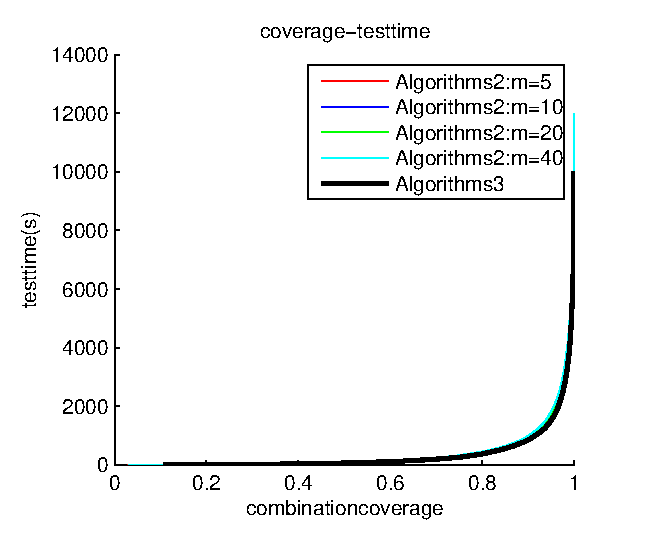
\includegraphics[width=2.5in,height=2.5in]{./a3_picture/coverage_testtime.eps}
   \caption{$coverage\_testtime$}
   \label{fig:ARCH}
 \end{figure}
%combination coverage good and bad\ref{fig:ARCH}
 \begin{figure}[htb]
   \centering
   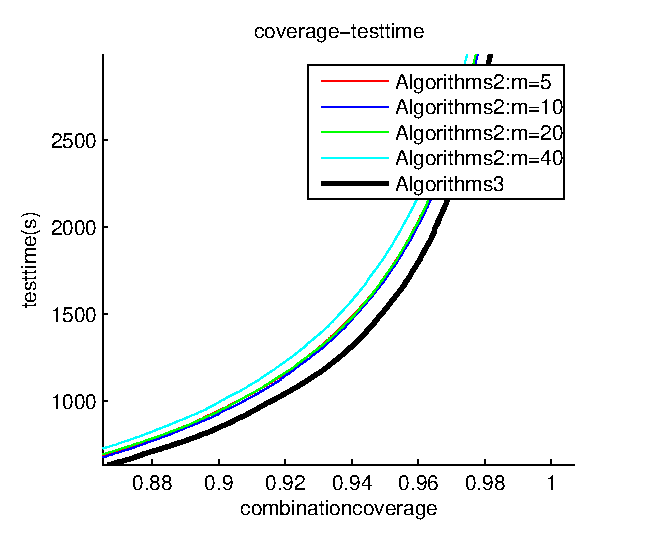
\includegraphics[width=2.5in,height=2.5in]{./a3_picture/coverage_testtime_enlarge.eps}
   \caption{$coverage\_testtime\_enlarge$}
   \label{fig:ARCH}
 \end{figure}

说明:横坐标为组合覆盖率,纵坐标为测试时间(原图和局部放大图),在相同组合覆盖率的时候,测试时间越
小说明效果越好,也就是横坐标相同,纵坐标越小越好

5 实验总结:根据以上结果可以看出,算法三花费的时间要小于算法二花费的时间,这就是算法三用到并行操作达到的效果,这正是我们想要的。
\end{CJK}
\end{document}
